\part{Weighted Digraphs and Optimization Problems}
\label{ch:weighted}


\chapter{Weighted graphs, the single-source shortest paths problem, Dijkstra} %----------

Weighted digrephs encode not only information about  \boldfont{whether} one can get from $A$ to $B$, but
\boldfont{how much it will cost} to do so.

The weight could represent the cost of using a link
in a communication network, or distance between nodes in a
transportation network. We use the terms of cost and distance
interchangeably.

We need a different ADT for this purpose. 

\section{Weighted digraphs}
\label{sec:weighted}

\begin{Definition}
A \defnfont{weighted digraph} is a pair $(G, c)$ where $G$ is a digraph
and $c$ is a \defnfont{cost function} associating a
real number to each arc of $G$. For an arc $(u,v)$, we interpret  $c(u, v)$ as the \defnfont{cost} of using $(u, v)$.
\end{Definition}

An ordinary digraph can be thought of as a special type of weighted digraph where the cost of each 
arc is $1$. 

%A weighted graph may be represented as a symmetric digraph where 
%each of a pair of antiparallel arcs has the same weight.

\begin{Boxample}
\label{ex:graphExWeighted}
A classic unweighted graph
(called the $3$-cube) of diameter $3$, a digraph with arc weights, and a
graph with edge weights.
\begin{center}
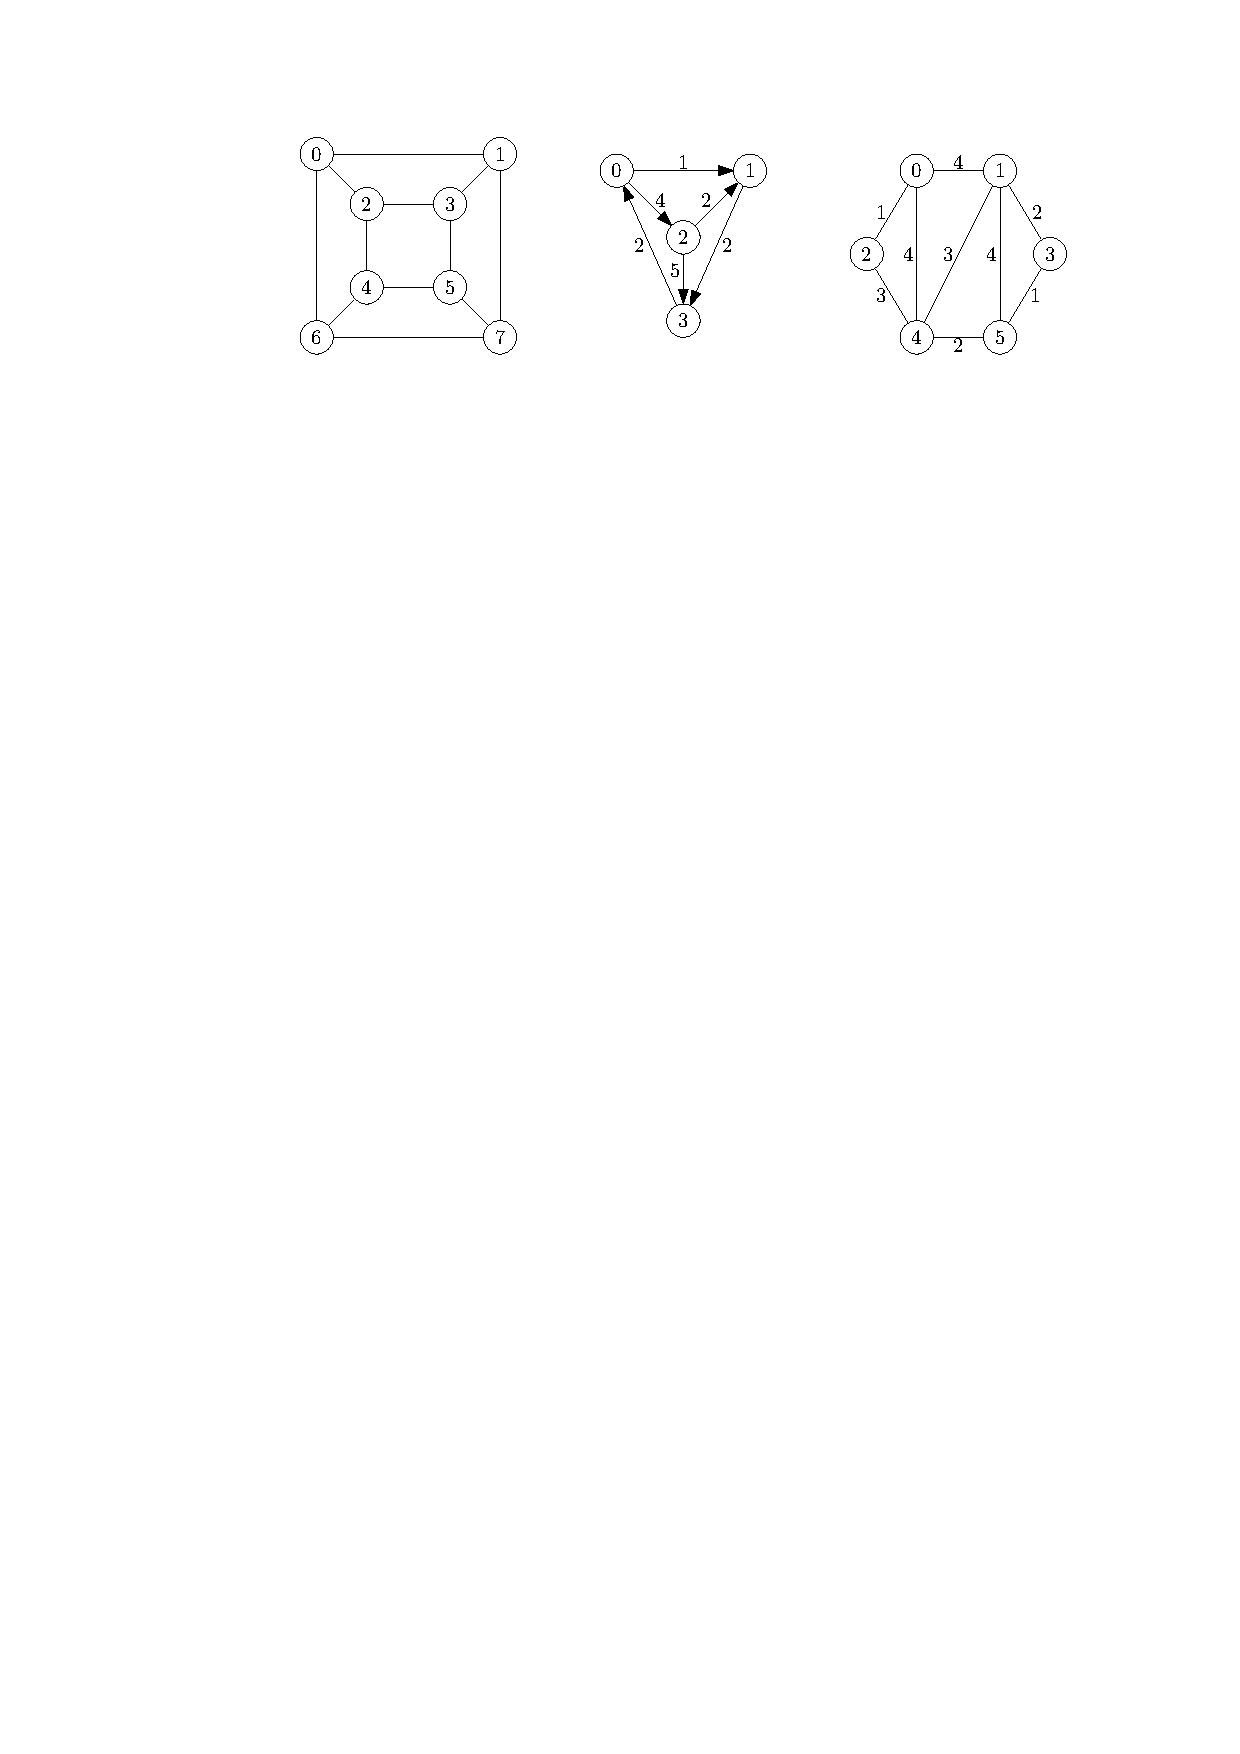
\includegraphics{graphExWeighted}
\end{center}
\end{Boxample}

Weighted digraphs can be represented using adjacency matrices or lists:
\begin{itemize}
\item The adjacency matrix is modified so that
each entry of $1$ (signifying that an arc exists) is replaced by the
cost of that arc.
\item Care needs to be taken if using 0 to represent the absence of arcs, as 0 may be a legal edge weight. 
In these cases, \texttt{null}, $\infty$ or some suitable value may be used.
\item We use \boldfont{the convention that 0 or null represents the absence of an arc. }
\item An adjacency list is modified so that the list associated  with node $v$ has each adjaceny node followed by the cost of the arc to the adjacent node. 
\item For example, the list for node 6 with adjacent arcs $(6,2)$ with $c(6,2) = 4$ and $(6,7)$ with $c(6,7) = 5$ would be $2,4,7,5$.
\end{itemize}

%If there is no arc between $u$ and $v$, then in an ordinary adjacency
%matrix the corresponding entry is $0$. However, in a weighted adjacency
%matrix, the ``cost" of a non-existent arc should be set consistantly 
%for most applications. We adopt the following \boldfont{convention}. 
%An entry of \verb|null| or $0$ in a weighted 
%adjacency matrix
%means that the arc does not exist, and vice versa. In many of our
%algorithms below, such entries should be replaced by the programming
%equivalent of \verb|null| for class objects, or $\infty$ for 
%primitive data types.  In the later case, we might use some positive 
%integer greater than any expected value that might occur during
%an execution of the program. 


\begin{Boxample}[1]
Draw the weighted graph given by the weighted adjacency matrix below. 
\newline

$
\left[
\begin{array}{cccc}
0 & 3 & 4 & 0  \\
3 & 0 & 1 & 3  \\
4 & 1 & 0 & 2  \\
0 & 3 & 2 & 0  \\
\end{array}
\right]
$
\vspace{1cm}


Draw the weighted digraph given by the weighted list representation below.
\newline

$
\AdjLists{
\begin{tabular}{c|llll}
0 & 1 & 3 & 2 & 4 \\
1 & 0 & 2 & 3 & 2 \\
2 & 1 & 3 &   &   \\
3 & 2 & 1 &   &   \\
\end{tabular}
}
$
\end{Boxample}

%See Appendix~\ref{sec:wgraphs} for sample Java code for representing
%the abstract data type of edge-weighted digraphs.

%\subsection*{Exercises}

\section{Distance and diameter in unweighted digraphs}\label{sec:unweighted}

Recall that the distance between nodes $u$ and $v$, $d(u,v)$ in a digraph, is simply the number of arcs in the shortest path between them. 

\begin{Definition}\label{def:diameter}
The \defnfont{diameter} of a strongly connected digraph $G$ is the
maximum of $d(u,v)$ over all nodes $u, v\in V(G)$. If the graph is not strongly connected the diameter is undefined though can be set to $\infty$.
\end{Definition}

%\begin{note} If the digraph is not strongly connected then the
%diameter is not defined; the only ``reasonable" thing it could be
%defined to be would be $+\infty$, or perhaps $n$ (since 
%no path in $G$ can have length more than $n-1$).
%\end{note}

%\begin{Example}
%The diameter of the $3$-cube in \cref{fig:graphExample5} is easily
%seen to be $3$. Since the digraph $G_2$ in \cref{fig:graphExample}
%is not strongly connected, the diameter is undefined.  
%\end{Example}

\begin{itemize}
\item It is often helpful to have the \defnfont{distance matrix} for a digraph.
The $(i, j)$-entry of this matrix contains the distance between node $i$
and node $j$.
\item Clearly the diameter is just the maximum entry in the distance matrix.
\item The distance matrix can be generated by running \algfont{BFSvisit}
from each node in turn, since the distance to a node is equal to its depth in the BFS tree (or infinte if the node is not reachable from the start node so not in the tree). This gives an algorithm with running time in $\Theta(n^2+nm)$.
\end{itemize}

\begin{Boxample}
A graph, its adjacency matrix and its distance matrix.\\

\begin{minipage}[c]{0.3\textwidth}
\centering
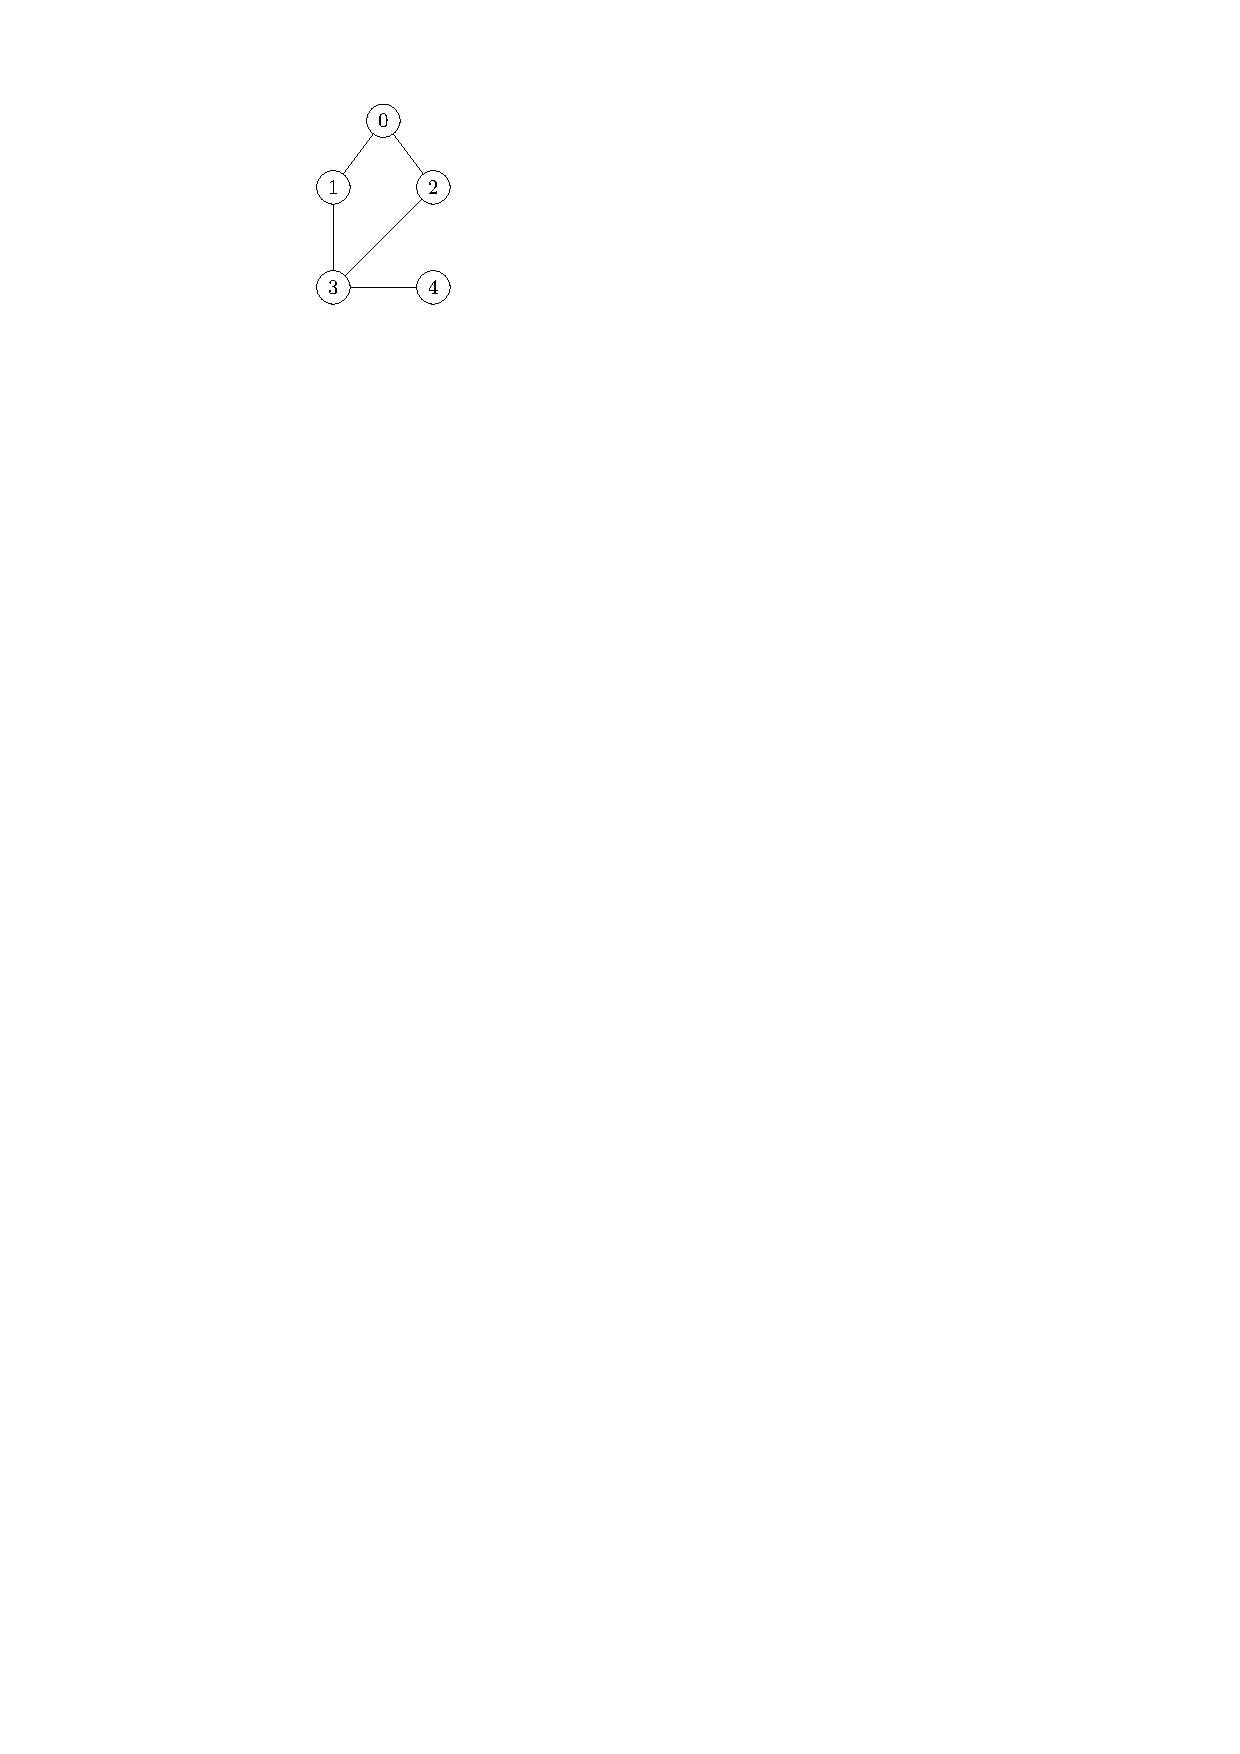
\includegraphics{distanceMatrixGraph}
\end{minipage}
\begin{minipage}[c]{0.65\textwidth}
$$\left[
\begin{array}{ccccc}
0 & 1 & 1 & 0 & 0 \\
1 & 0 & 0 & 1 & 0 \\
1 & 0 & 0 & 1 & 0 \\
0 & 1 & 1 & 0 & 1 \\
0 & 0 & 0 & 1 & 0 \\
\end{array}
\right]
\hspace{2cm}
\left[
\begin{array}{ccccc}
0 & 1 & 1 & 2 & 3 \\
1 & 0 & 2 & 1 & 2 \\
1 & 2 & 0 & 1 & 2 \\
2 & 1 & 1 & 0 & 1 \\
3 & 2 & 2 & 1 & 0 \\
\end{array}
\right]$$
\end{minipage} 
\end{Boxample}

% \begin{Example}
% An adjacency matrix and a distance matrix for the 3-cube shown in
% \cref{fig:graphExample5} is given below.  The maximum entries of
% value $3$ indicate the diameter. The reader should check these entries
% by performing a breadth-first search from each vertex.
% \[
% \left[
% \begin{array}{cccccccc}
% 0& 1& 1& 0& 0& 0& 1& 0\\
% 1& 0& 0& 1& 0& 0& 0& 1 \\
% 1& 0& 0& 1& 1& 0& 0& 0\\
% 0& 1& 1& 0& 0& 1& 0& 0 \\
% 0& 0& 1& 0& 0& 1& 1& 0 \\
% 0& 0& 0& 1& 1& 0& 0& 1 \\
% 1& 0& 0& 0& 1& 0& 0& 1 \\
% 0& 1& 0& 0& 0& 1& 1& 0 \\
% \end{array}
% \right]
% \hspace{2cm}
% \left[
% \begin{array}{cccccccc}
% 0& 1& 1& 2& 2& 3& 1& 2\\
% 1& 0& 2& 1& 3& 2& 2& 1\\
% 1& 2& 0& 1& 1& 2& 2& 3\\
% 2& 1& 1& 0& 2& 1& 3& 2\\
% 2& 3& 1& 2& 0& 1& 1& 2\\
% 3& 2& 2& 1& 1& 0& 2& 1\\
% 1& 2& 2& 3& 1& 2& 0& 1\\
% 2& 1& 3& 2& 2& 1& 1& 0\\
% \end{array}
% \right]
% \]
% \end{Example}


%\subsection*{Exercises}

\begin{Boxample}[2]
Give an example of a weighted digraph in which the BFS approach
does not find the shortest path from the root to a node.
\end{Boxample}

%\begin{Exercise}
%\label{ex:radius}
%The \defnfont{eccentricity} of a node $u$ in a  digraph $G$  is the
%maximum of $d(u, v)$ over all $v\in V(G)$. The \defnfont{radius} of $G$
%is the minimum eccentricity of a node. Write an
%algorithm to compute the radius of a digraph in time $\Theta(n^2 +
%nm)$. How can we read off the radius from a distance matrix?
%\end{Exercise}

\section{Single-source shortest path problem}
\label{sec:SSSP}

In  the \defnfont{single-source shortest path} problem (SSSP) we are given a weighted digraph $(G, c)$ and a source node
$s$. 
For each node $v$ of $G$, we must find the minimum weight of a path
from $s$ to $v$ (by the weight of a path we mean the sum of the weights
on the arcs). This is like  finding row $s$ in a weighted distance matrix.

\begin{Boxample} \label{eg:SSSP}
In the weighted digraph pictured, the unique minimum weight path from $0$ to $3$ is $0, 1, 3$ with weight $3$.
What is the minimum weight path from $2$ to $0$, what is its weight?\\

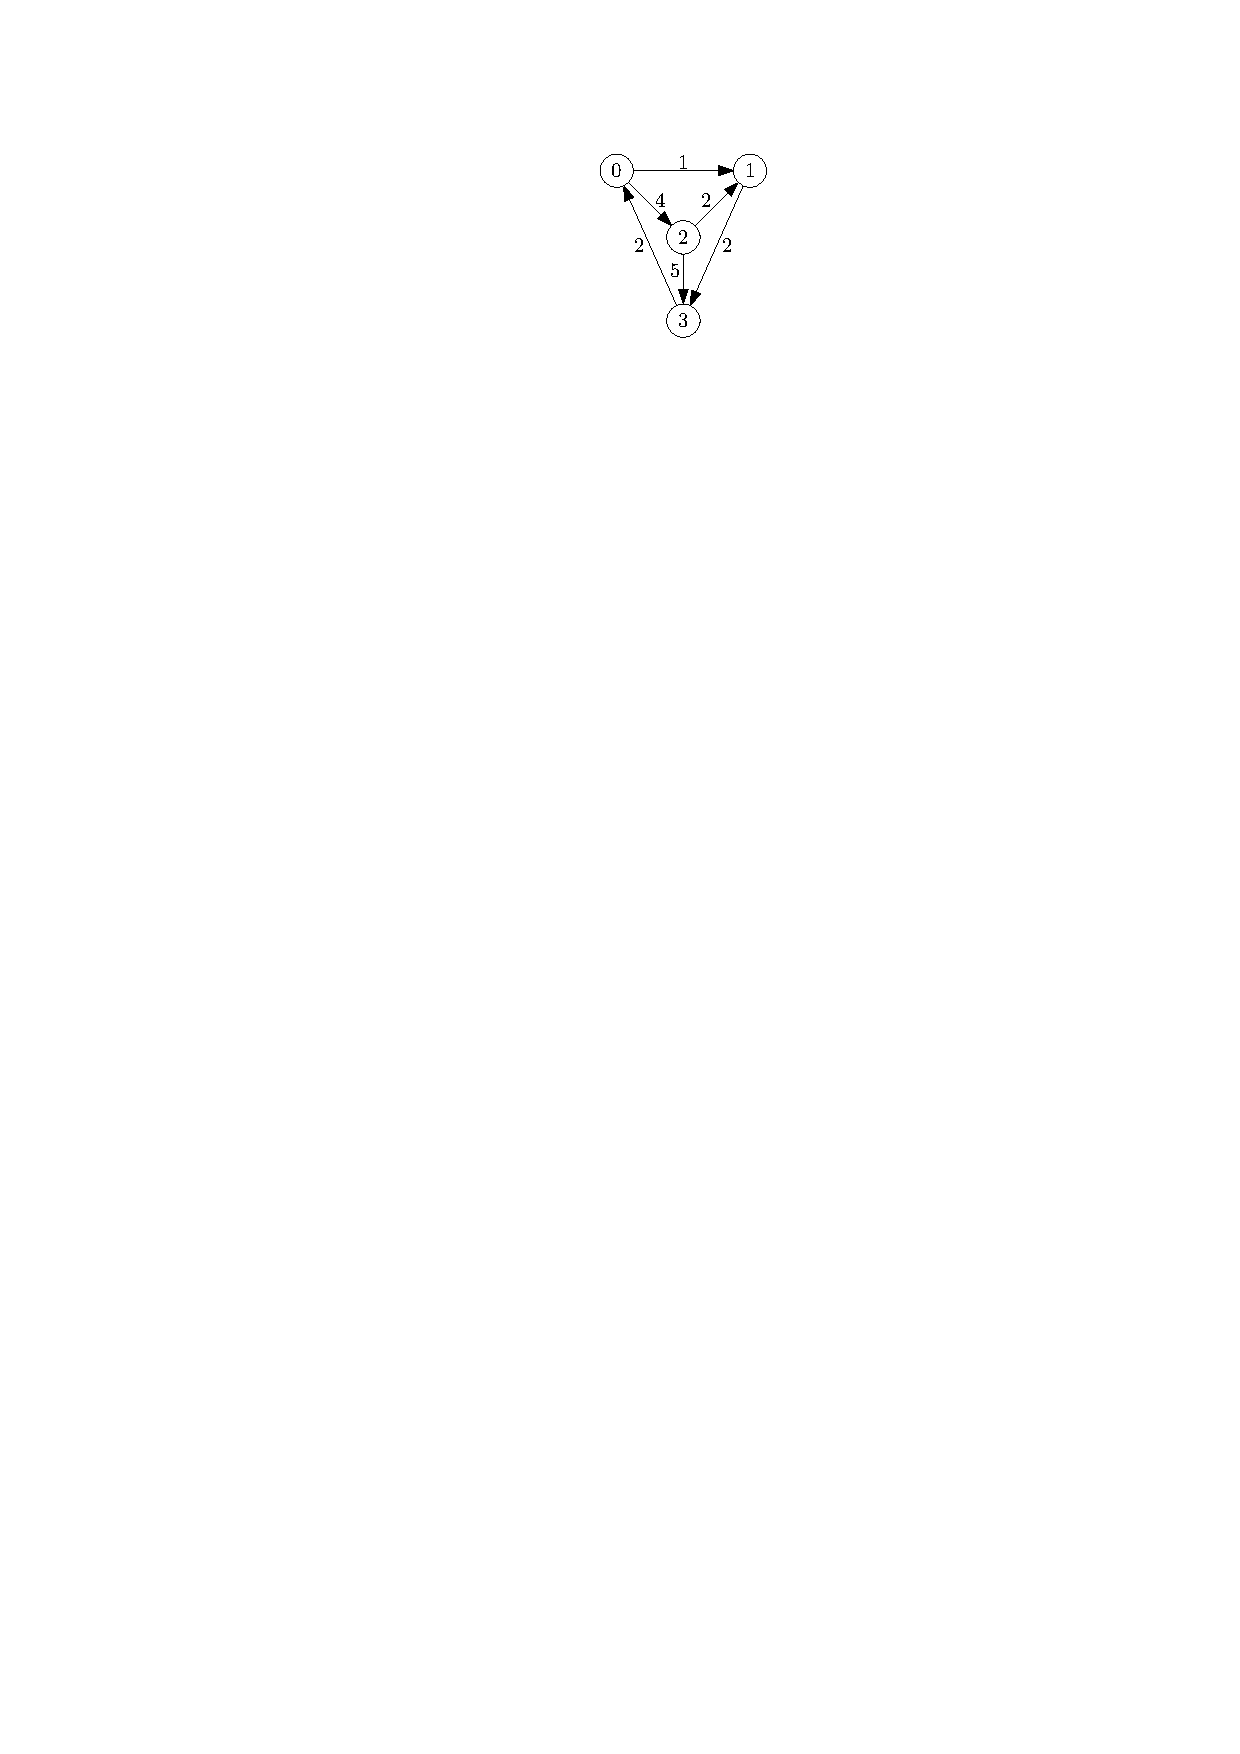
\includegraphics{weightedDigraph}
\end{Boxample}

\section{Dijkstra's algorithm}
Dijkstra's algorithm solves the SSSP problem whenever \boldfont{all weights are nonnegative}. It may fail in the presence of negative weight arcs.


It is easiest to understand the algorithm in terms of a set of visited nodes, $S$, which eventually includes all nodes in $G$. We'll consider only shortest paths through $S$ and make sure the length of these shortest paths is accurate. Once $S = V(G)$, all shortest path lengths are known. 

Initially $S$ contains only the
single node $s$. The only paths available are the one-arc paths from $s$ to neighbours 
$v$, of weight $c(s, v)$. We choose the neighbour $u$ with $c(s, u)$ minimal and
add it to $S$. 

Now the fringe nodes adjacent to $s$ and $u$ must be
updated to reflect possible paths  through $u$ (it is possible that there
exists a path from $s$ to $v$, passing through $u$, that is shorter
than the direct path from $s$). 
Now we choose the node %(at ``level" $1$ or $2$) 
whose current best distance to $s$ is smallest, and update
again. We continue in this way until all nodes belong to $S$.

%The basic structure of the algorithm is presented in
In \cref{alg:dijkstra}, the set $S$ consists of the BLACK nodes.


\begin{algorithm}[H]
  \caption{Dijkstra's algorithm (first version)}
    \label{alg:dijkstra}
\begin{algorithmic}[1]
\Function{Dijkstra}{weighted digraph $(G, c)$; node $s\in V(G)$}
	\State array $\colour[0..n-1]$, $\dist[0..n-1]$
	\For{$u \in V(G)$}
		\State $\dist[u] \gets c[s,u]$; $\colour[u] \gets$ WHITE 
	\EndFor
	\State $\dist[s] \gets 0$; $\colour[s] \gets $ BLACK
	\While{there is a white node}
		\State find a white node $u$ so that $\dist[u]$ is minimum
		\State $\colour[u] \gets $ BLACK
		\For{$x \in V(G)$}
			\If{$\colour[x] = $ WHITE}
				\State $\dist[x] \gets \min \{\dist[x], \dist[u] + c[u,x]\}$  
			\EndIf
		\EndFor
	\EndWhile
	\State \Return{$\dist$}
\EndFunction
\end{algorithmic}
\end{algorithm}

\begin{Boxample}
An application of Dijkstra's algorithm with starting vertex $0$. 
The distances to 0 at each step are displayed next to each node.
\begin{center}
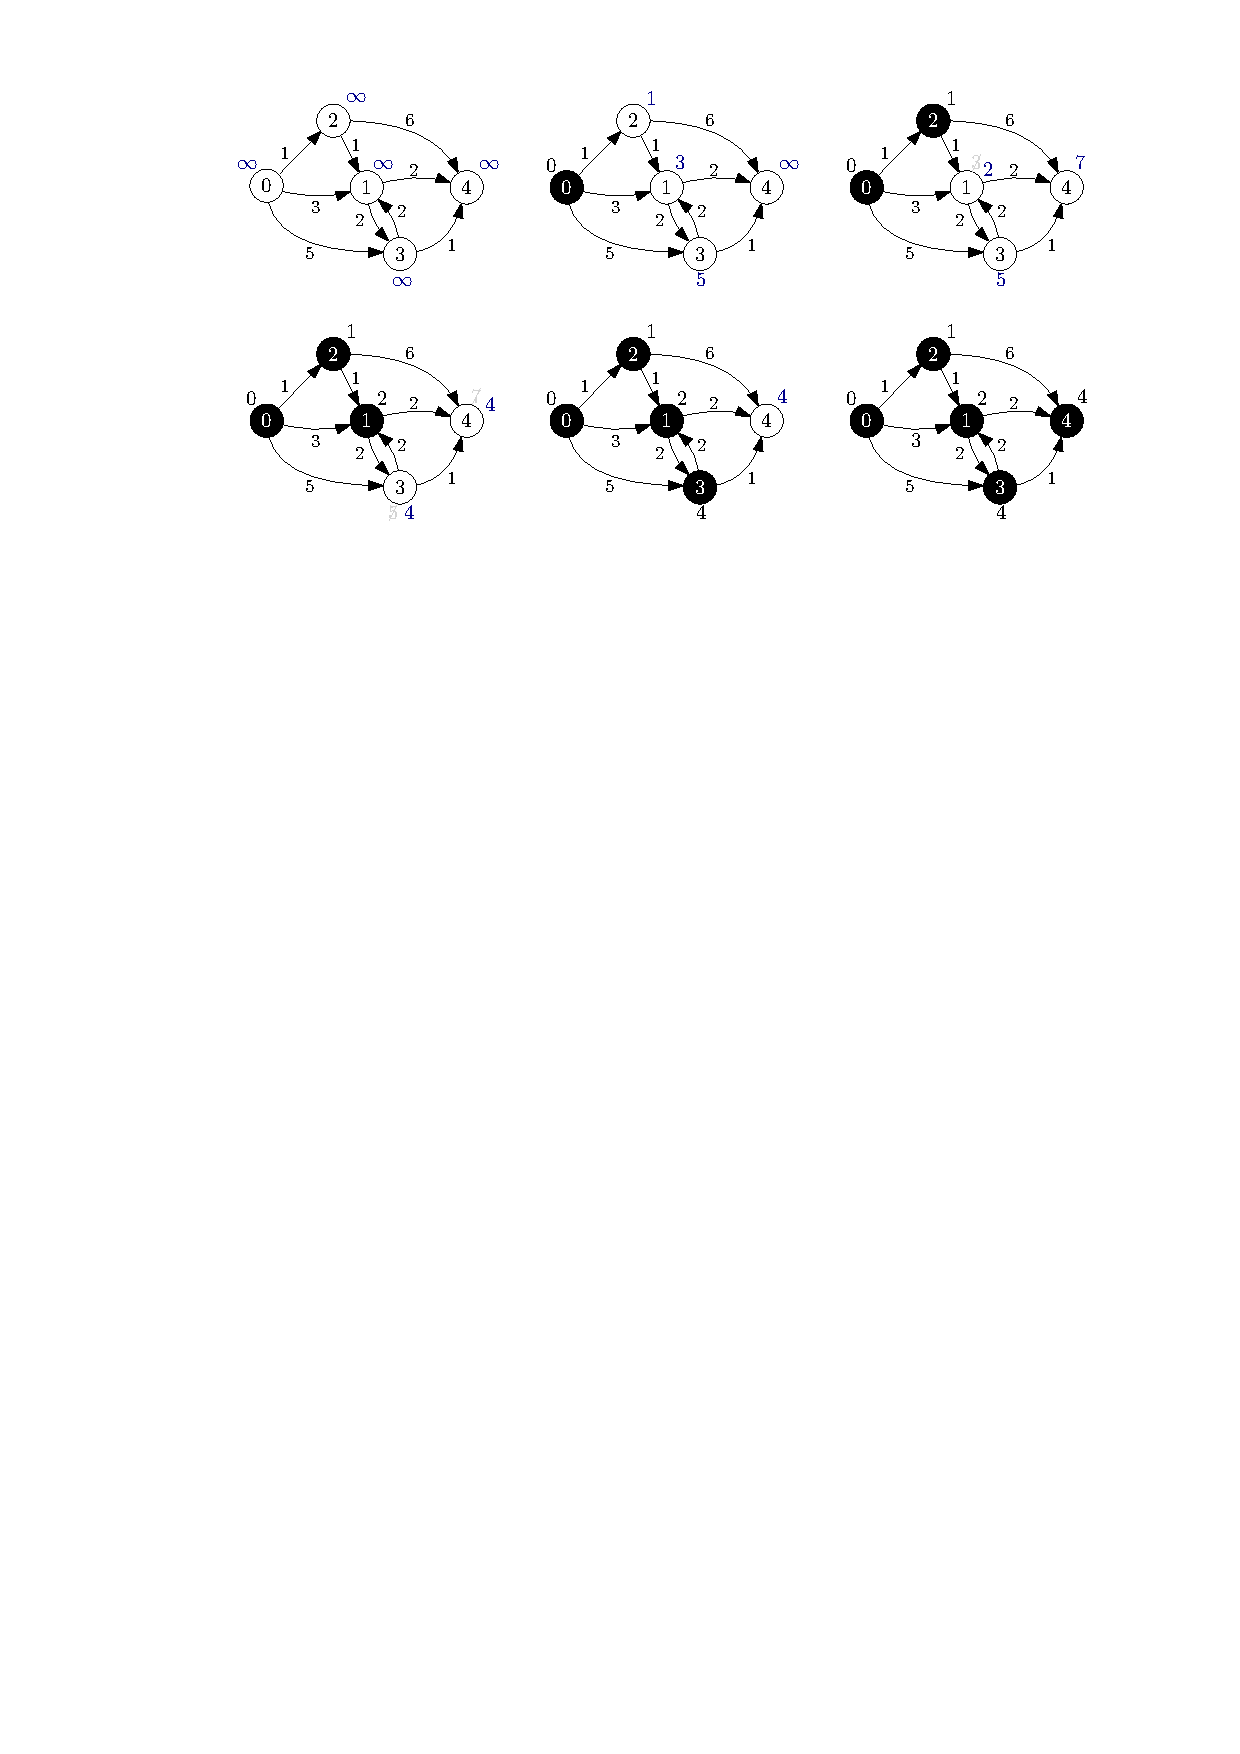
\includegraphics[width=1.0\textwidth]{DijkstraEx}
\end{center}
\end{Boxample}

\begin{Boxample}\mbox{}\\
\label{ex:dijs-all-vert}
\begin{minipage}[c]{0.45\textwidth}
An application of Dijkstra's algorithm on the digraph below
for each starting vertex $s$. 
Complete the table for the starting vertex 2.

\begin{center}
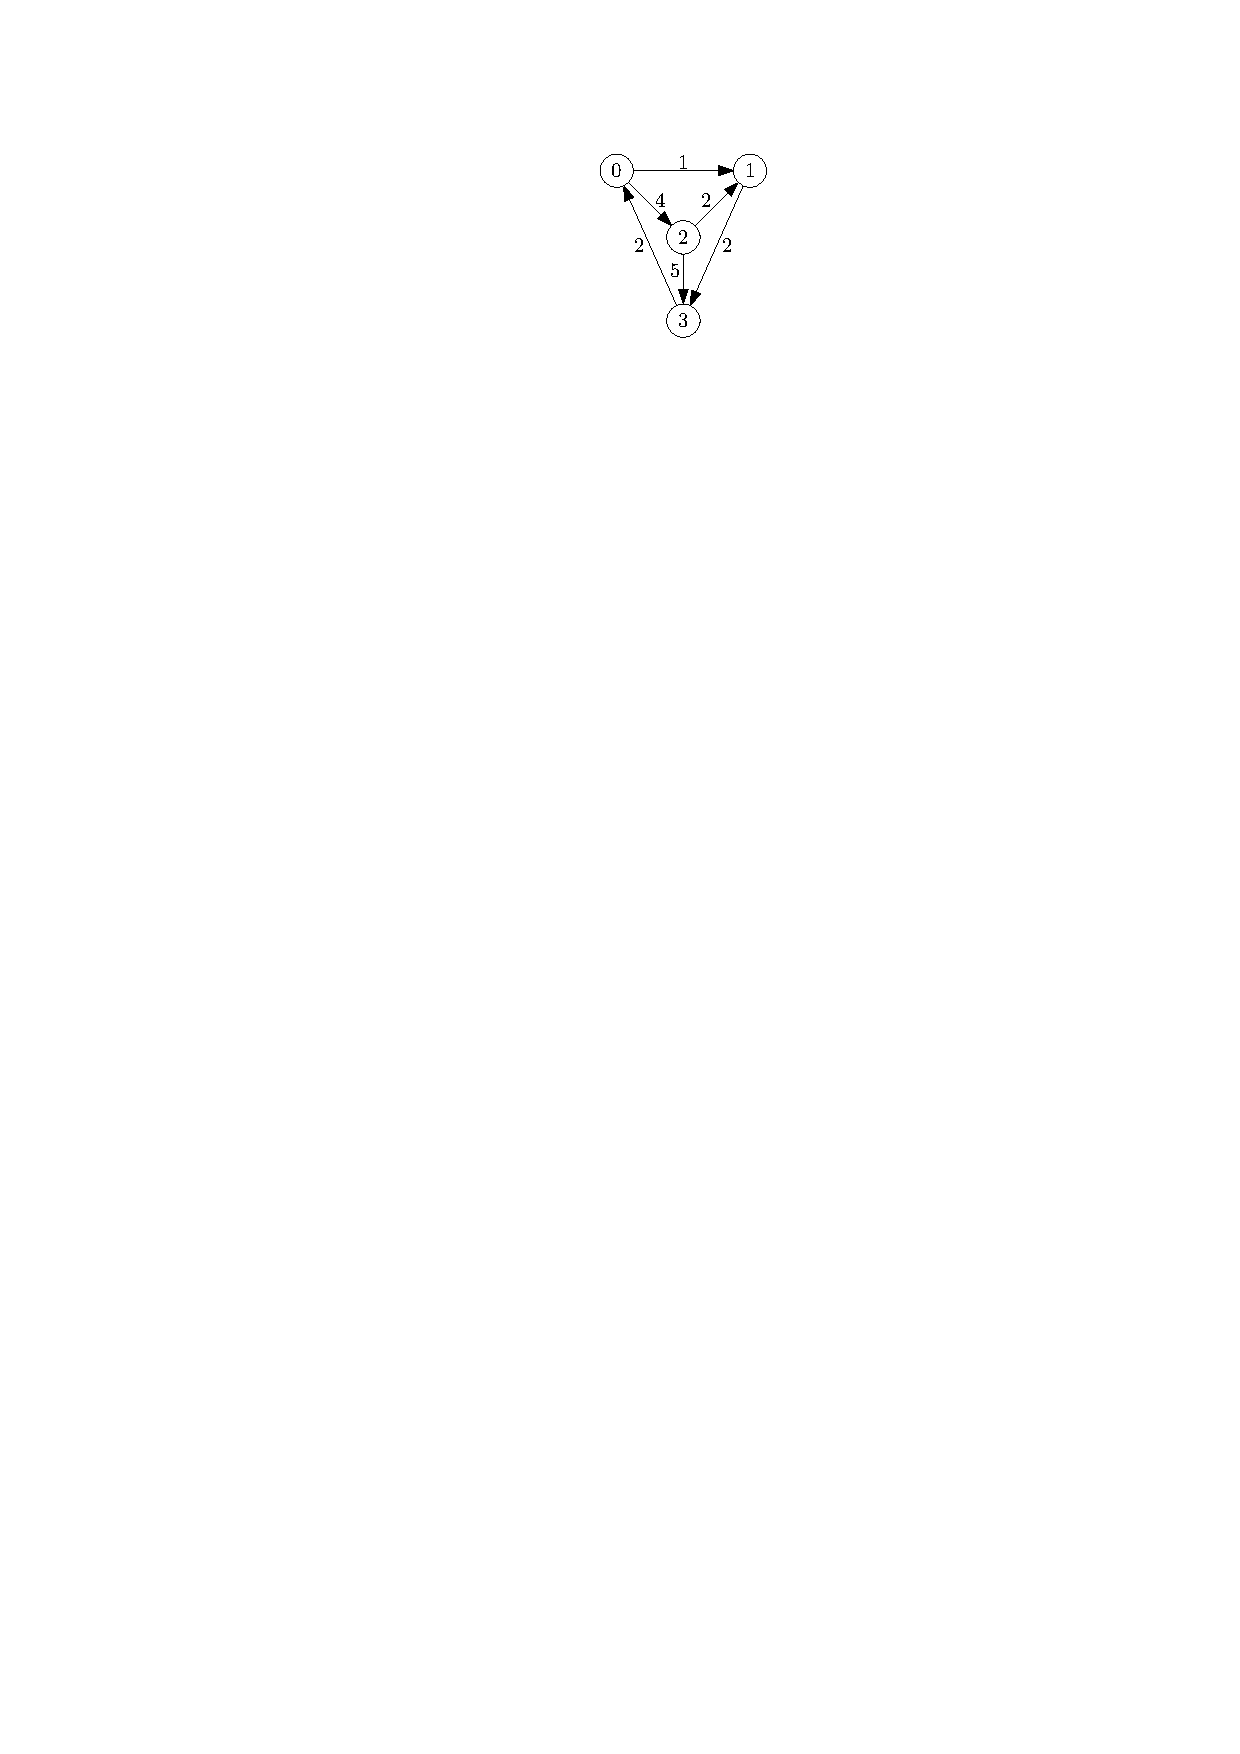
\includegraphics{weightedDigraph}
\end{center}

The table illustrates that the distance vector is updated at 
most $n - 1$ times (only before a new vertex is selected and added to $S$). 
Thus we could have omitted the lines with $S = \set{0,1,2,3}$.
\end{minipage}$\quad$
\begin{minipage}[c]{0.45\textwidth}
\begin{tabular}{|c|c|}\hline
\textbf{current} $S \subseteq V$ &  \textbf{distance vector} $\dist$  \\ \hline
\set{0} & $0, 1, 4, \infty$  \\
\set{0,1} & $0, 1, 4, 3$  \\
\set{0,1,3} & $0, 1, 4, 3$  \\
\set{0,1,2,3} & $0, 1, 4, 3$  \\ \hline
\set{1} & $\infty, 0, \infty, 2$  \\
\set{1,3} & $4, 0, \infty, 2$ \\
\set{0,1,3} & $4, 0, 8, 2$ \\
\set{0,1,2,3} & $4, 0, 8, 2$ \\ \hline
\set{2} & \\%$\infty, 2, 0, 5$  \\
&\\
\set{1,2} & \\%$\infty, 2 , 0, 4$ \\
&\\
\set{1,2,3} & \\%$6, 2, 0, 4$  \\
&\\
\set{0,1,2,3} & \\ %\hline %$6, 2, 0, 4$ \\ \hline
&\\ \hline
\set{3} & $2, \infty, \infty, 0$ \\
\set{0,3} & $2, 3, 6, 0$ \\
\set{0,1,3} & $2, 3, 6, 0 $ \\
\set{0,1,2,3} & $2, 3, 6, 0$ \\ \hline
\end{tabular}
\end{minipage}\\
\end{Boxample}



\chapter{Dijkstra proof and running time} %--------------------------------------

\begin{Boxample}[0.5] \label{ex:dijk-neg-fails}
Dijkstra's algorithm may fail to give the correct answer if some weights are negative.
Give weights to the edges of the digraph below such that running Dijkstra's algorithm with starting vertex $0$
fails. 
\vspace{0.5cm} 
\begin{center}
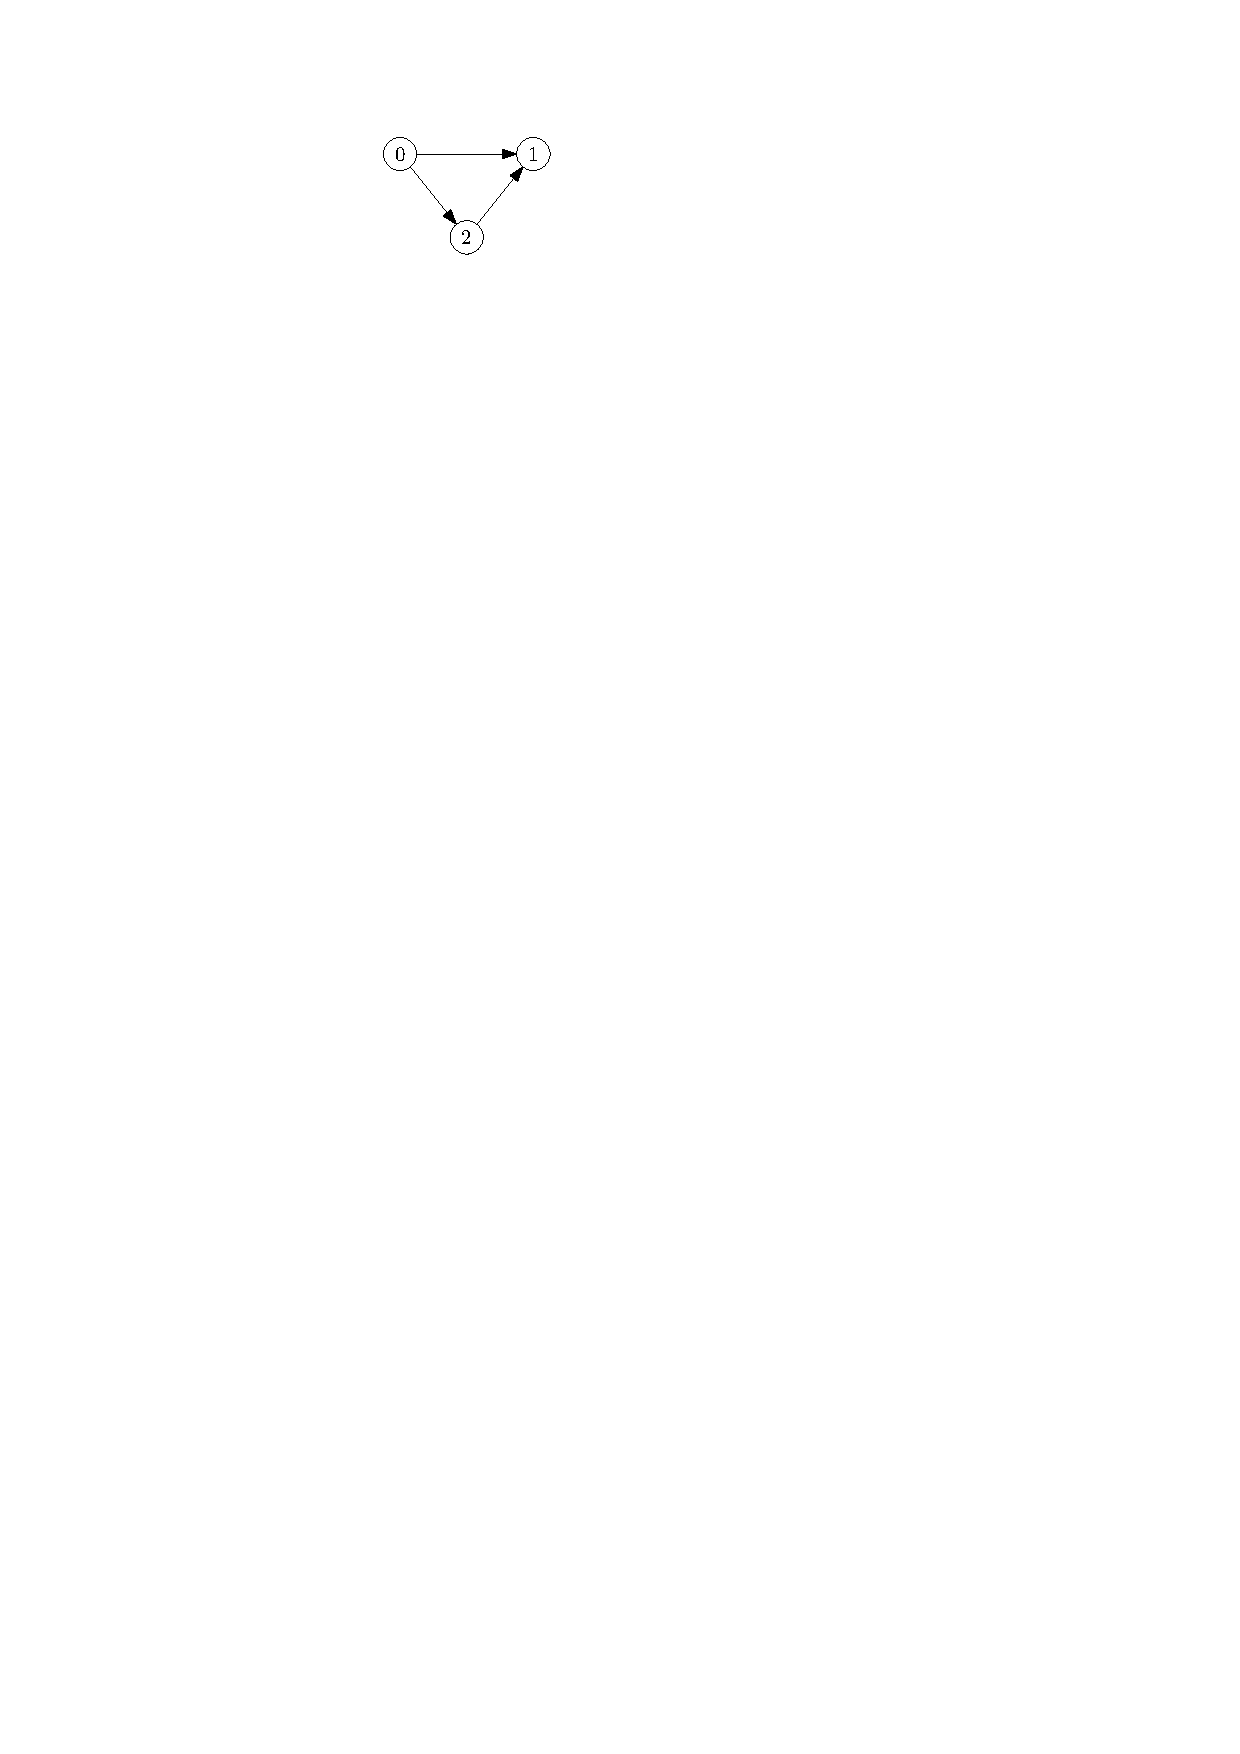
\includegraphics{DijkstraTriangle}
\end{center}
% Give an example to show that Dijkstra's algorithm may fail to give the correct answer 
% if some weights are negative. Make your example as small as possible. 
% Then run the Bellman--Ford algorithm on the example and verify that it gives the correct answer.
\end{Boxample}


Proving that Dijkstra's algorithm works is a little more tricky than others we've seen.

Define an \defnfont{$\boldsymbol S$-path} from $s$ to $w$ as a
path from $s$ to $w$ with all intermediate nodes belonging to $S$. In other words, $w$ may not belong to $S$, but all other nodes in the path do.

\begin{Theorem}
\label{thm:dijkstra} Suppose that all arc weights are nonnegative. Then
at the top of the \boldfont{while} loop, we have the following properties:
\begin{description}
\item[P1:] if $x\in V(G)$, then $\dist[x]$ is the minimum cost of an $S$-path 
from $s$ to $x$;
\item[P2:] if $w\in S$, then $\dist[w]$ is the minimum cost of a path
from $s$ to $w$.
\end{description}
\end{Theorem}

\begin{note} Assuming the result to be true for a moment, we can see
that once a node $u$ is added to $S$ and $\dist[u]$ is updated, $\dist[u]$
never changes in subsequent iterations. When the algorithm terminates,
all nodes belong to $S$ and hence $\dist$ holds the correct distance information.
\end{note}
\begin{proof} 
Note that at every step, $\dist[x]$ does contain
the length of \boldfont{some} path from $s$ to $x$; that path is an
$S$-path if $x\in S$. Also, the update formula ensures that $\dist[x]$
never increases. 

To prove P1 and P2, we use induction on the number of times $k$ we
have been through the while-loop. Let $S_k$ denote the value of $S$
at this stage. When $k=0$, $S_0=\{s\}$, and since $\dist[s]=0$, P1 and
P2 obviously hold. Now suppose that they hold after $k$ times through
the while-loop and let $u$ be the next special node chosen during that
loop. Thus $S_{k+1} = S_k \cup \set{u}.$

We first show that P2 holds after $k+1$ iterations. Suppose that
$w\in S_{k+1}$.  If $w\neq u$ then $w\in S$ and so P2 trivially
holds for $w$ by the inductive hypothesis. On the other hand,
if $w=u$, consider any $S_{k+1}$-path $\gamma$ from $s$ to $u$.
%(see \cref{fig:dijk-proof1}). 
We shall show that $\dist[u] \leq
|\gamma |$ where $| \gamma | $ denotes the weight of $\gamma$. The
last node before $u$ is some $y\in S_k$. Let $\gamma_1$ be the subpath
of $\gamma$ ending at $y$. Then $\dist[u] \leq \dist[y] + c(y,u)$ by the
update formula. Furthermore $\dist[y] \leq |\gamma_1 |$ by the inductive
hypothesis applied to $y\in S_k$. Thus, combining these inequalities,
we obtain $\dist[u] \leq |\gamma_1 | + c(y, u) = | \gamma |$ as
required. Hence P2 holds for every iteration.

Now suppose $x\in V(G)$. Let $\gamma$ be any $S_{k+1}$-path to $x$. If
$u$ is not involved then $\gamma$ is an $S_k$ path and so $|\gamma| \leq
\dist[x]$ by the inductive hypothesis. Now suppose that $\gamma$ does
include $u$. 
If $\gamma$ goes straight from $u$ to $x$, we let $\gamma_1$ denote the 
subpath of $\gamma$ ending at $u$. Then $|\gamma| = |\gamma_1| + c(u,x) \geq 
\dist[x]$ by the update formula. 
Otherwise, after reaching $u$, the path returns into $S_k$
directly, emerging from $S_k$ again, at some node $y$ before going
straight to $x$ (see \cref{fig:dijk-proof2}). Let $\gamma_1$
be the subpath of $\gamma$ ending at $y$. Since P2 holds for $S_k$,
there is a minimum weight $S_k$-path $\beta$ from $s$ to $y$ of length
$\dist[y]$. Thus by the update formula, 
$$
|\gamma| = |\gamma_1| + c(y,
x) \geq |\beta| + c(y, x) \geq \dist[y] + c(y, x) \geq \dist[x].
$$ 
Hence P1 holds for all iterations.
\end{proof}

Dijkstra's algorithm is an example of a \defnfont{greedy algorithm}. 
At each step it makes the best choice involving only local information,
and never regrets its past choices. 

jo TODO: suggestions to improve this proof? And the figure is not working here...(not sure it is the best figure.)

\begin{figure}
%\centerline{\input{figs/wDijkstra.pstex_t}}
\caption{Picture for proof of Dijkstra's algorithm.}
\label{fig:dijk-proof2}
\end{figure}

\section{Running time of Dijkstra}

The study of the time complexity of Dijkstra's algorithm leads to many
interesting topics.

Note that the value of $\dist[x]$ will change only if $x$ is adjacent to
$u$. Thus if we use a weighted adjacency list, the block inside the
second for-loop need only be executed $m$ times. However, if
using the adjacency matrix representation, the block inside the for-loop
must still be executed $n^2$ times.

The time complexity is of order $a n + m$ if adjacency lists are used,
and $a n + n^2$ with an adjacency matrix, where $a$ represents the time
taken to find the node with minimum value of $\dist$. The obvious method
of finding the minimum is simply to scan through array $\dist$
sequentially, so that $a$ is of order $n$, and the running time of
Dijkstra is therefore $\Theta(n^2)$. Dijkstra himself originally used
an adjacency matrix and scanning of the $\dist$ array. 


\chapter{Dijkstra and PFS, Bellman-Ford algorithm}

\section{PFS implementation of Dijkstra}
\begin{itemize}
\item We can implement Dijkstra's algorithm using priority-first search ideas. 
\item The key value associated to a node $u$ is simply the
value $\dist[u]$, the current best distance to that node from the root $s$.
\end{itemize}

\begin{algorithm}[H]
  \caption{Dijkstra's algorithm, PFS version.}
  \label{alg:dijkstra2}
\begin{algorithmic}[1]
\Function{Dijkstra2}{weighted digraph $(G, c)$; node $s \in V(G)$}
	\State priority queue $Q$
	\State array $\colour[0..n-1]$, $\dist[0..n-1]$
	\For{$u \in V(G)$}
		\State $\colour[u] \gets$ WHITE 
	\EndFor
	\State $\colour[s] \gets $ GREY
	\State $Q$.\algfont{insert}$(s, 0)$
	\While{\textbf{not} $Q$.\algfont{isEmpty}$()$}
		\State $u \gets Q$.\algfont{peek}$()$; $t_1 \gets$  $Q$.\algfont{getKey}$(u)$
		\For{each $x$ adjacent to $u$}
			\State $t_2 \gets t_1 + c(u, x)$
			\If{$\colour[x] = $ WHITE}
				\State $\colour[x] \gets $ GREY
				\State $Q$.\algfont{insert}$(x, t_2)$
			\ElsIf{$\colour[x] = $ GREY \textbf{and} $Q$.\algfont{getKey}$(x) > t_2$}
				\State $Q$.\algfont{decreaseKey}$(x, t_2)$
			\EndIf
		\EndFor
		\State $Q$.\algfont{delete}$()$
		\State $\colour[u] \gets $ BLACK
		\State $\dist[u] \gets t_1$ 
	\EndWhile
	\State \Return{$\dist$}
\EndFunction
\end{algorithmic}
\end{algorithm}


This formulation makes it clear that we need to perform $n$
delete-min operations and at most $m$ decrease-key operations, and
that these dominate the running time. Hence using a binary heap, Dijkstra's
algorithm runs in time $O((n + m) \log n)$. Thus if every node is reachable 
from the source, it runs in time $O(m\log n)$.

%The quest to improve the complexity of algorithms like Dijkstra's has
%led to some very sophisticated data structures that can implement the
%priority queue in such a way that the decrease-key operation is faster
%than in a heap, without sacrificing the delete-min or other operations.
%Many such data structures have been found, mostly complicated variations
%on heaps; some of them are called Fibonacci heaps and 2--3 heaps. 

Specialised data structures to implement priority queues can improve the running time of Dijktra's.

The best complexity bound for Dijkstra's algorithm, using a \emph{Fibonacci heap},
is $O(m + n\log n)$.



\section{Bellman--Ford algorithm} \label{sec:bellford}

\begin{itemize}
\item Bellman--Ford solve the SSSP problem even when there are negative weight arcs
\item It  runs more slowly than Dijkstra's 
\item  The basic idea, as with Dijkstra's algorithm, is to solve the SSSP under  restrictions
that become progressively more relaxed. 
\item  Bellman--Ford solves the problem for all
nodes at ``level" $0, 1, \dots , n-1$ in turn.
\item  By level we mean the
minimum possible number of arcs in a minimum weight path to that node from the
source.
\end{itemize}

\begin{algorithm}[H]
  \caption{Bellman--Ford algorithm.}
  \label{alg:bellford-code}
\begin{algorithmic}[1]
\Function{BellmanFord}{weighted digraph $(G, c)$; node $s \in V(G)$}
	\State array $\dist[0..n-1]$
	\For{$u \in V(G)$}
		\State $\dist[u] \gets \infty$ 
	\EndFor
	\State $\dist[s] \gets 0$
	\For{$i$ \textbf{from} $0$ \textbf{to} $n-1$}
		\For{$x \in V(G)$}
			\For{$v \in V(G)$}
				\State $\dist[v] \gets \min( \dist[v], \dist[x] + c(x,v) )$
			\EndFor
		\EndFor
	\EndFor
	\State \Return{$\dist$}
\EndFunction
\end{algorithmic}
\end{algorithm}

\begin{Boxample}[0]
An application of Bellman--Ford algorithm with starting vertex $4$
when the nodes are processed in the order from $0$ to $4$.
\begin{center} 
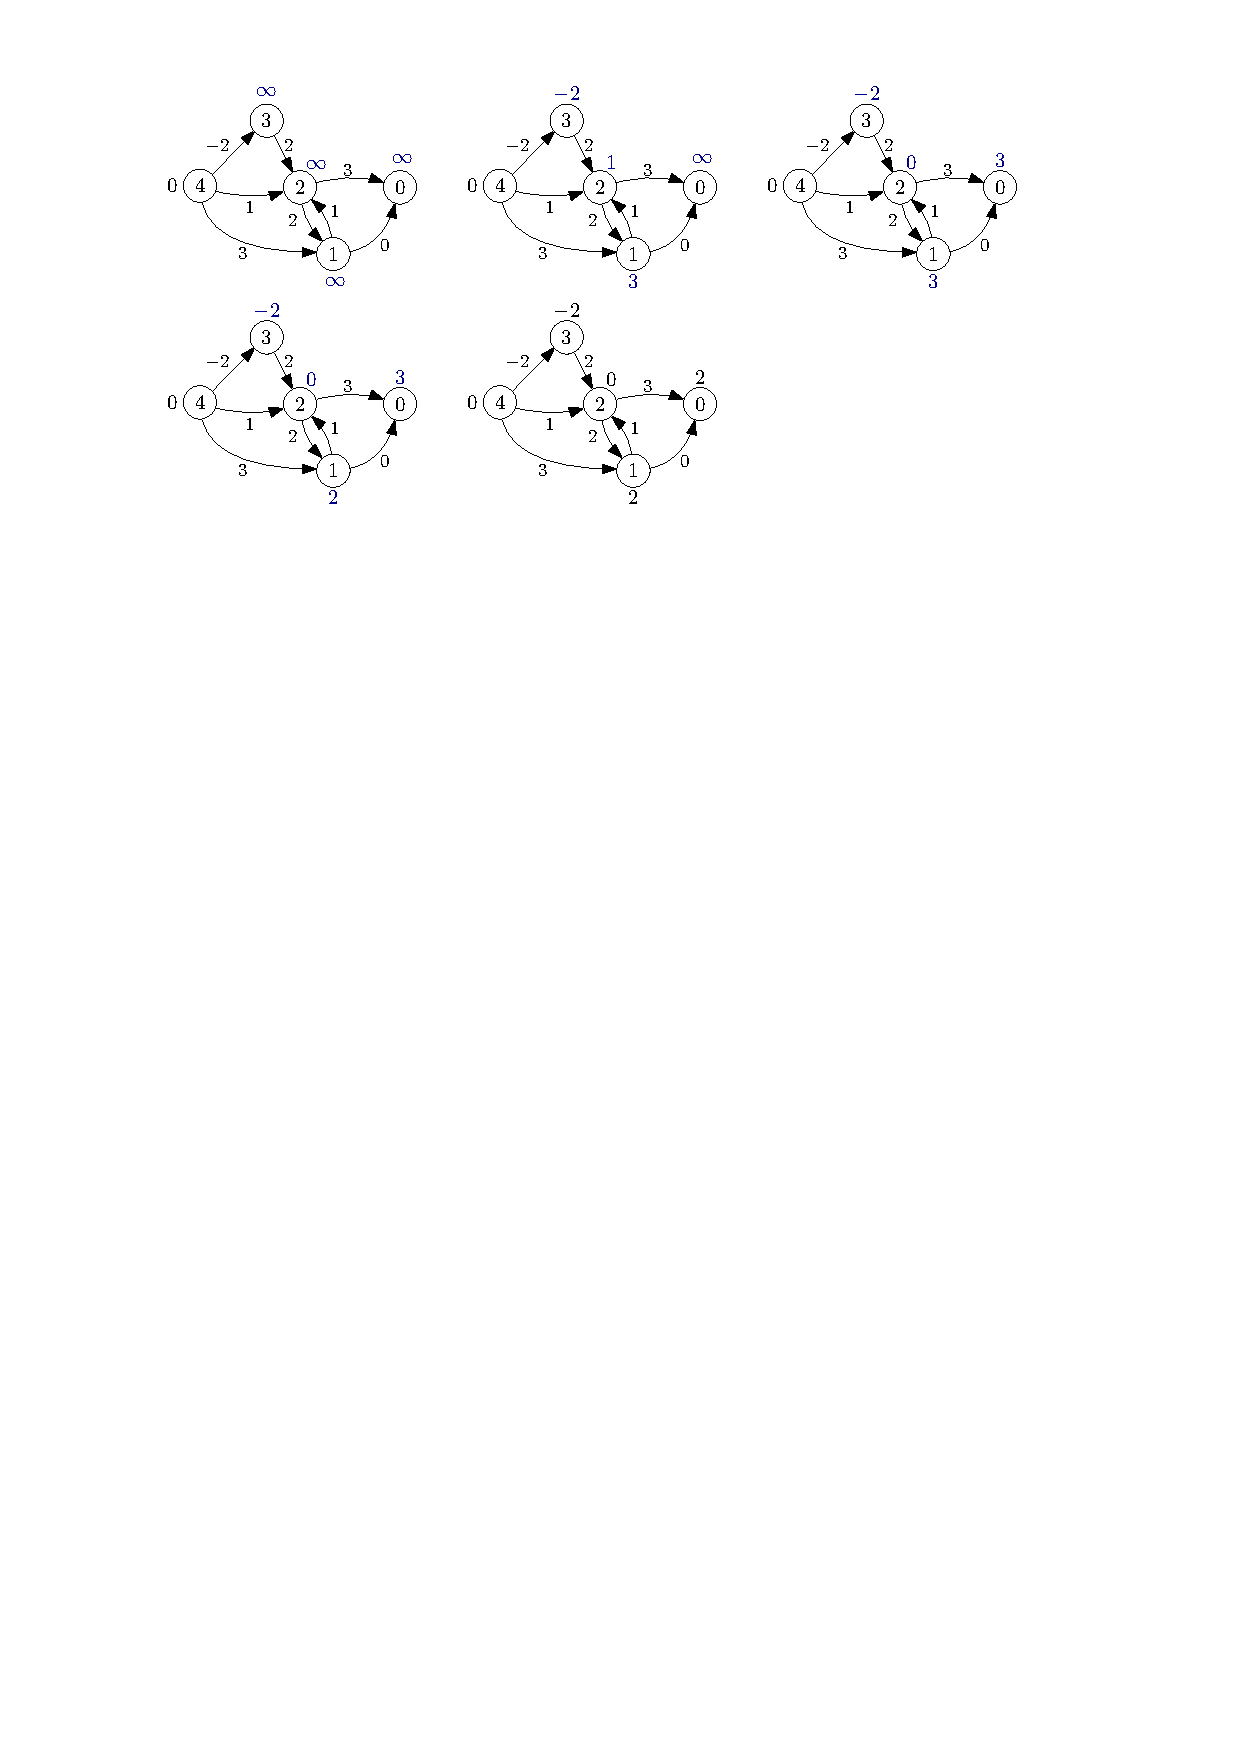
\includegraphics[width=1.0\textwidth]{BellmanFordEx}
\end{center}
%After how many iterations would the algorithm converge to the exact distance, 
%if the nodes are processed in the order $4$, $3$, $2$, $1$, $0$?
\end{Boxample}

\begin{Theorem} 
Suppose that $G$ contains no negative weight cycles. Then after the $i$-th 
iteration of the outer for-loop, $\dist[v]$ contains the minimum weight of a 
path to $v$ for all nodes $v$ with level at most $i$.
\end{Theorem}

\begin{proof} 
Note that as for Dijkstra, the update formula is such that
$\dist$ values never increase.

We use induction on $i$. When $i=0$ the  result is true because of our
initialization. Suppose it is true for $i-1$. Let $v$ be a node at level
$i$, and let $\gamma$ be a minimum weight path from $s$ to $v$. Since
there are no negative weight cycles, $\gamma$ has $i$ arcs. If $y$
is the last node of $\gamma$ before $v$, and $\gamma_1$ the subpath to
$y$, then by the inductive hypothesis we have $\dist[y] \leq | \gamma_1
|$. Thus by the update formula we have $\dist[v] \leq \dist[y] + c(y, v)
\leq | \gamma_1 | + c(y, v) \leq | \gamma |$ as required.
\end{proof}

The Bellman--Ford algorithm runs in time $\Theta(nm)$ using adjacency
lists, since the statement in the inner for-loop need only be
executed if $v$ is adjacent to $x$, and the outer loop runs $n$
times. Using an adjacency matrix it runs in time $\Theta(n^3)$.

\subsection*{Exercises}

%\newpage
% \begin{Exercise} 
% \label{ex:do-bellford}
% Run the Bellman--Ford algorithm on the digraph with weighted adjacency 
% matrix given below. Choose each node as the source in turn as in 
% Example~\ref{eg:dijkstra}.
% $$
% \left[
% \begin{matrix}
% 0 & 6 & 0 & 0 & 7 \\
% 0 & 0 & 5 & -4 & 8 \\
% 0 & -2 & 0 & 0 & 0 \\
% 2 & 0 & 7 & 0 & 0 \\
% 0 & 0 & -3 & 9 & 0 \\
% \end{matrix}
% \right]
% $$
% \end{Exercise}

\begin{Boxample}[2] \label{ex:SSSP-neg-cycle}
Explain why the SSSP problem makes no sense if we allow digraphs with
cycles of negative total weight.
\end{Boxample}

%\newpage
% \begin{Exercise}\label{ex:dijk-SI} % maybe use for assignment (on North Island)?
% The graph shows minimum legal driving times (in multiples of 5 minutes) 
% between various South Island towns. What is the shortest time to drive legally from
% Picton to (a) Wanaka, (b) Queenstown and (c) Invercargill? Explain which
% algorithm you use and show your work.
% \begin{center}
% 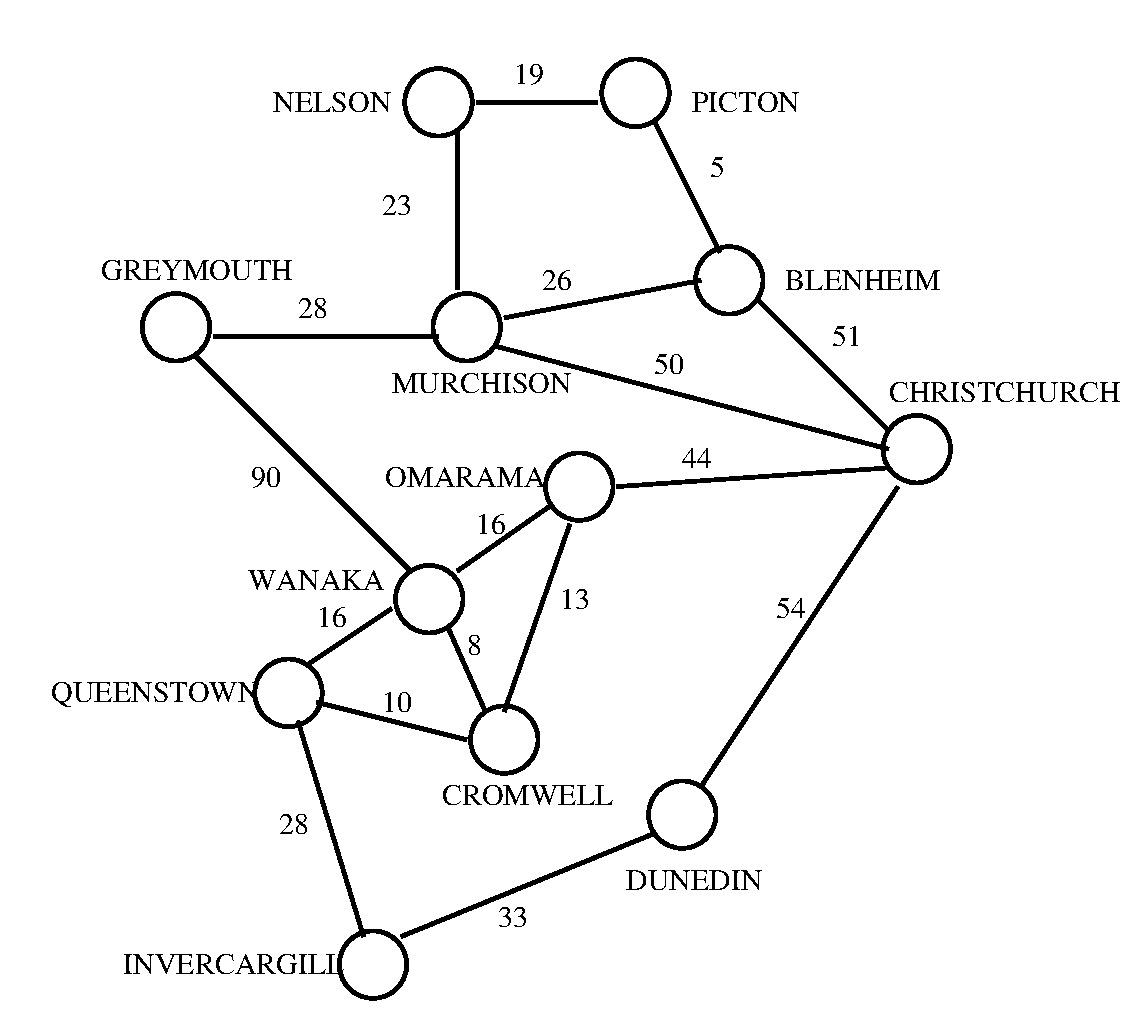
\includegraphics[width=8cm]{southisland}
% %\verb|\epsfig{figure=figs/SI.xfg.eps, width=12cm}|
% \end{center}
% \end{Exercise}

\begin{Boxample}[2]\label{ex:bellman-neg-cycle}
Suppose the input to the Bellman--Ford algorithm is a digraph with a
negative weight cycle. How could the algorithm detect this, so it can
exit gracefully with an error message?
\end{Boxample}


% \begin{Exercise}
% \label{ex:dijk-proof}
% Where in the proof of Dijkstra's algorithm do we use the fact that 
% all the arc weights are nonnegative?
% \end{Exercise}



\chapter{All-pairs shortest path problem} %-----------------------------------
\label{sec:APSP}

In the \defnfont{all-pairs shortest path} (APSP) problem we are given a weighted digraph $(G, c)$, and must determine 
for each $u, v\in V(G)$ the weight of a minimum weight path from $u$
to $v$.

The solution to all-pairs shortest path can be presented as a distance matrix.

\begin{Boxample}[0]
\label{eg:APSP}
For the digraph we have already
calculated the all-pairs distance matrix in \cref{ex:dijs-all-vert}:

jo TODO: how do we use cref for boxamples?

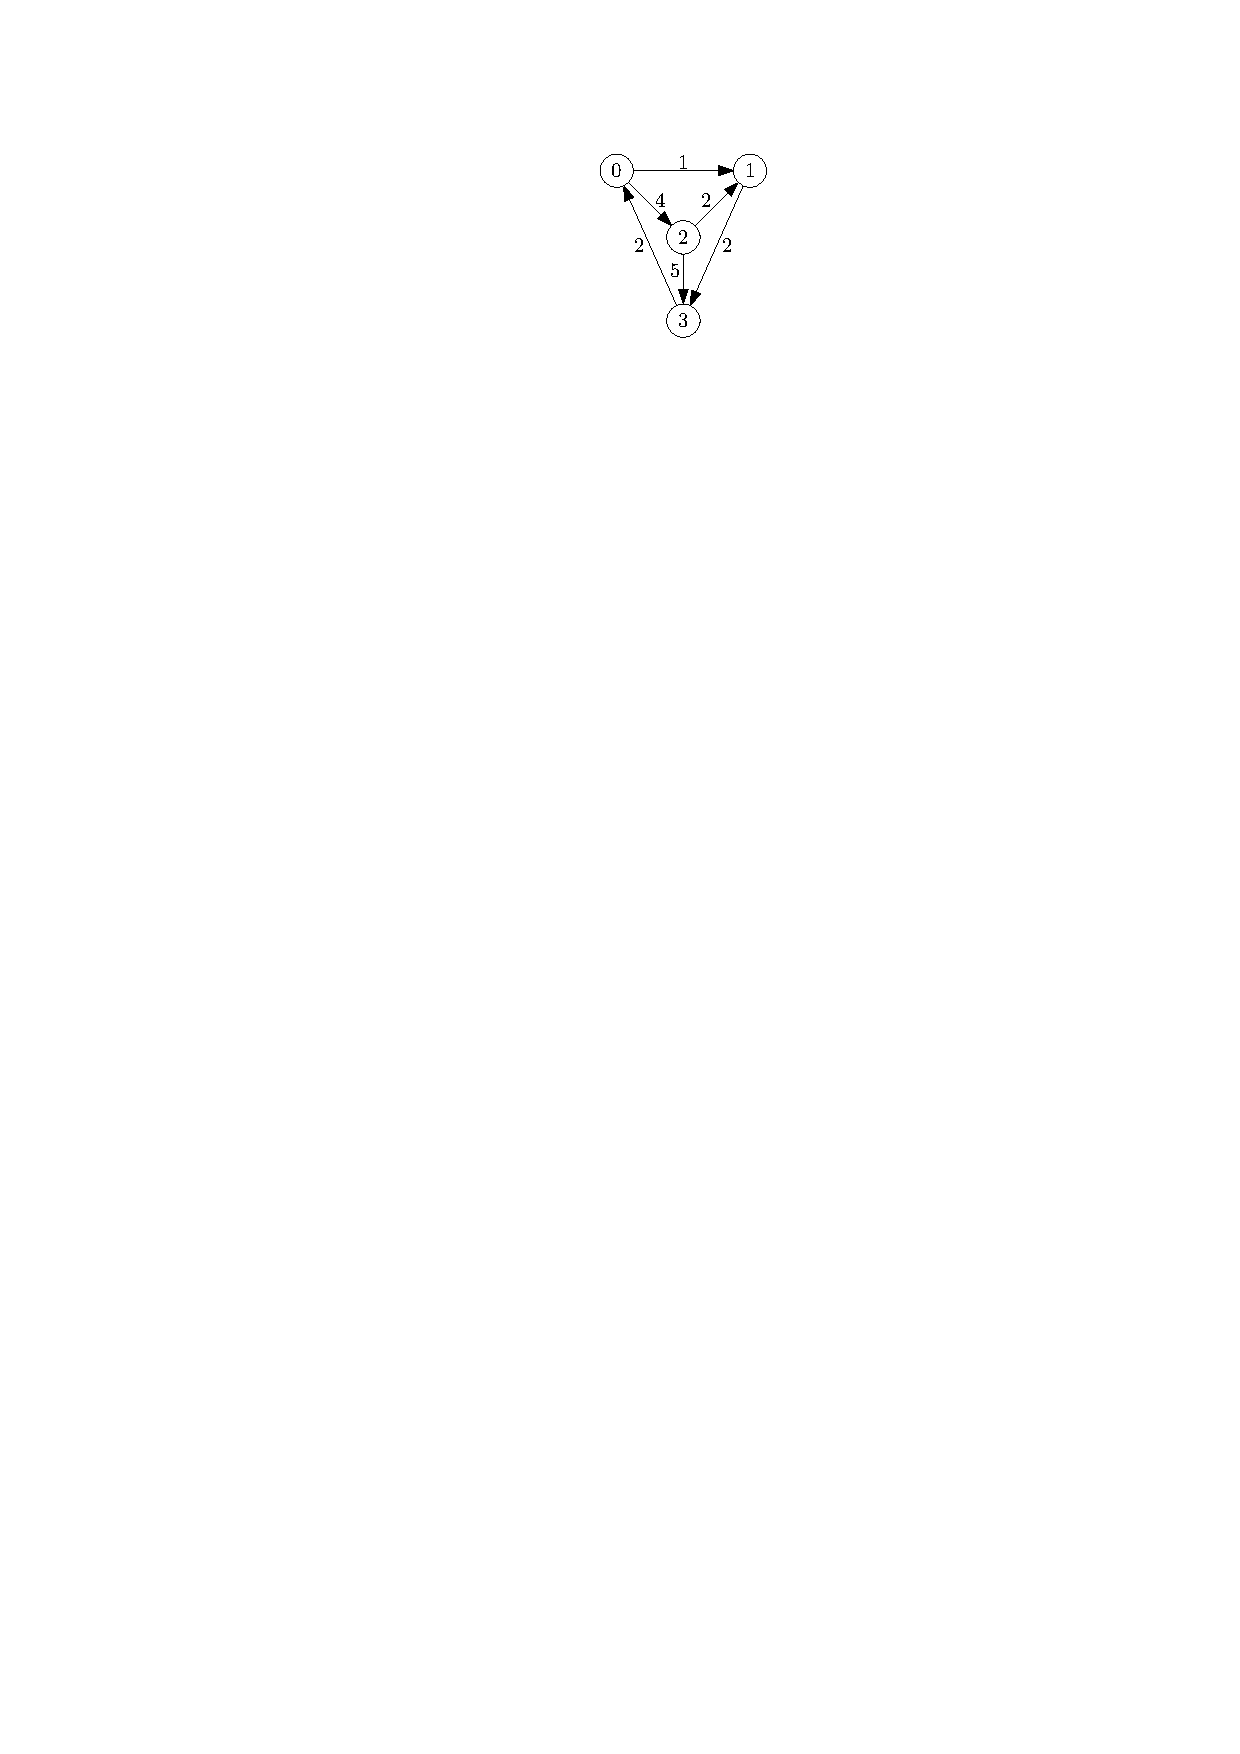
\includegraphics{weightedDigraph}
$$
\left(
\begin{matrix}
0 & 1 & 4 & 3 \\
4 & 0 & 8 & 2 \\
6 & 2 & 0 & 4 \\
2 & 3 & 6 & 0
\end{matrix}
\right).
$$
\end{Boxample}

\begin{itemize}
\item The APSP problem can be solved by solving the SSSP problem from each node.
\item If all weights were non-negative, we could run Dijsktra from each of the $n$ nodes, to get a running time of $\Theta(n^3)$.
\item To be robust to negative weights, using Bellman--Ford gives a $\Theta(n^2 m)$ solution to APSP.
\item \defnfont{Floyd's algorithm} computes a distance matrix
from a cost matrix (so solves ASPS) in time $\Theta(n^3)$. 
It is robust to negative weights. 
\item Floyd's is thus faster than Bellman--Ford for non-sparse digraphs.
\item It is essentially just a triple for-loop so easy to programme.
\end{itemize}

The basic idea behind Floyd's algorithm is that we find the length of the shortest path between nodes $u$ and $v$ that uses only a fixed set of intermediate nodes. This set of intermediate nodes starts at as the empty set (so only acrs from $u$ to $v$ are allowed) and grows, one node at a time, until it includes all nodes at which point the allgorithm is complete.

We see this in the pseudo-code where the outer-for loop interates through all nodes, essentially adding them to the intermediate set, while the inner two loops cycle through all pairs seeing if a shorter path can be found through the new intermediate node.

\begin{algorithm}[H]
  \caption{Floyd's algorithm.}
  \label{alg:floydcode}
\begin{algorithmic}[1]
\Function{Floyd}{weighted digraph $(G, c)$}
	\State array $d[0..n-1,0..n-1]$ \Comment{initialise distance matrix}
	\State $d \gets c$ \Comment{distance matrix starts as copy of weight matrix}
	\For{$x \in V(G)$} \Comment{taking one vertex at a time}
		\For{$u \in V(G)$}
			\For{$v \in V(G)$}
				\State $d[u,v] \gets \min( d[u,v], d[u,x] + d[x,v] )$ \Comment{update distance by looking for a shorter path through $x$}
			\EndFor
		\EndFor
	\EndFor
	\State \Return{$d$}
\EndFunction
\end{algorithmic}
\end{algorithm}


\begin{Boxample}[0]
\label{eg:floyd}
An application of Floyd's algorithm on the third graph of
\cref{ex:graphExWeighted} is given below.  The initial cost 
matrix is as follows.

\[ 
\left[
\begin{array}{cccccc} % cost matrix
0        & 4        & 1        & \infty & 4        & \infty \\
4        & 0        & \infty & 2        & 3        & 4 \\
1        &  \infty  & 0        &  \infty  & 3        &  \infty  \\
 \infty  & 2        &  \infty  & 0        &  \infty  & 1 \\
4        & 3        & 3        &  \infty  & 0        & 2 \\
 \infty  & 4        &  \infty  & 1        & 2        & 0 \\
\end{array}
\right]
\hspace{.5cm}
\]

In the matrices below, the index $k$ refers to
the number of times we have been through the outer for-loop.

\begin{samepage}
{\footnotesize
%
\[
\left[
\begin{array}{cccccc} % k = 0
0        & 4        & 1        &  \infty  & 4        &  \infty  \\
4        & 0        & \textbf{5}    & 2        & 3        & 4 \\
1        & \textbf{5}    & 0        &  \infty  & 3        &  \infty  \\
 \infty  & 2        &  \infty  & 0        &  \infty  & 1 \\
4        & 3        & 3        &  \infty  & 0        & 2 \\
 \infty  & 4        &  \infty  & 1        & 2        & 0 \\
\end{array}
\right]
\hspace{.5cm}
\left[
\begin{array}{cccccc} % k = 1
0        & 4        & 1        & \textbf{6}    & 4     & \textbf{8} \\
4        & 0        & 5        & 2        & 3        & 4 \\
1        & 5        & 0        & \textbf{7}    & 3      & \textbf{9} \\
\textbf{6}    & 2        & \textbf{7}    & 0        & \textbf{5}  & 1 \\
4        & 3        & 3        & \textbf{5}    & 0        & 2 \\
\textbf{8}   & 4        & \textbf{9}    & 1        & 2        & 0 \\
\end{array}
\right]
\hspace{.5cm}
\left[
\begin{array}{cccccc} % k = 2
0    & 4   & 1   & 6    & 4    & 8 \\
4    & 0   & 5   & 2    & 3    & 4 \\
1    & 5   & 0   & 7    & 3    & 9 \\
6    & 2   & 7   & 0    & 5    & 1 \\
4    & 3   & 3   & 5    & 0    & 2 \\
8    & 4   & 9   & 1    & 2    & 0 \\
\end{array}
\right]
\]\\[-5pt]
\hspace*{1in}$k=1$ \hspace{1.2in} $k=2$ \hspace{1.2in} $k=3$ \\
\[
\left[
\begin{array}{cccccc} % k = 3
0    & 4   & 1   & 6    & 4    & \textbf{7} \\
4    & 0   & 5   & 2    & 3    & \textbf{3} \\
1    & 5   & 0   & 7    & 3    & \textbf{8} \\
6    & 2   & 7   & 0    & 5    & 1 \\
4    & 3   & 3   & 5    & 0    & 2 \\
\textbf{7} &\textbf{3} & \textbf{8} & 1    & 2    & 0 \\
\end{array}
\right]
\hspace{.5cm}
\left[
\begin{array}{cccccc} % k = 4
0    & 4   & 1     & 6    & 4    & \textbf{6} \\
4    & 0   & 5     & 2    & 3    & 3 \\
1    & 5   & 0     & 7    & 3    & \textbf{5} \\
6    & 2   & 7     & 0    & 5    & 1 \\
4    & 3   & 3     & 5    & 0    & 2 \\
\textbf{6} & 3   & \textbf{5} & 1    & 2    & 0 \\
\end{array}
\right]
\hspace{.5cm}
\left[
\begin{array}{cccccc} % k = 5
0    & 4   & 1     & 6    & 4    & 6 \\
4    & 0   & 5     & 2    & 3    & 3 \\
1    & 5   & 0     & \textbf{6} & 3    & 5 \\
6    & 2   & \textbf{6} & 0    & \textbf{3} & 1 \\
4    & 3   & 3     & \textbf{3} & 0    & 2 \\
6    & 3   & 5     & 1    & 2    & 0 \\
\end{array}
\right]
\]\\[-5pt]
\hspace*{1in} $k=4$ \hspace{1.2in} $k=5$ \hspace{1.2in} $k=6$
\\
} % footnotesize
\end{samepage}

In the above matrices we list the entries that change in bold after each
increment of $k$. 
\end{Boxample}

\section{Proof of Floyd's algorithm}

\begin{Theorem}
\label{thm:floyd}
At the bottom of the outer \boldfont{for} loop, for all nodes $u$ and $v$,
$d[u,v]$ contains the minimum length of all paths from $u$ to $v$ that
are restricted to using only intermediate nodes that have been seen in
the outer \boldfont{for} loop. 
\end{Theorem}

%\begin{note}
%Given this fact, when the algorithm terminates, all nodes have been seen
%in the outer \boldfont{for} loop and so $d[u,v]$ is the length of a
%shortest path from $u$ to $v$.
%\end{note}

\begin{proof}
To establish the above property, we use induction on the outer for-loop.
Let $S_k$ be the set of nodes seen after $k$ times through the
outer loop, and define an $S_k$-path  to be one all of whose
intermediate nodes belong to $S_k$. The corresponding value of $d$ is 
denoted $d_k$. We need to show that for all $k$, after $k$ times through 
the outer for-loop, $d_k[u,v]$ is the minimum length of an $S_k$-path 
from $u$ to $v$. 

When $k=0$, $S_0 = \emptyset$ and the result holds. Suppose
it is true after $k$ times through the outer loop and consider what
happens at the end of the $(k+1)$-st time through the outer loop.
Suppose that $x$ was the last node seen in the outer loop, so $S_{k+1}=
S_k \cup \{x\}$. Fix $u, v\in V(G)$ and let $L$ be the minimum length of
an $S_{k+1}$-path from $u$ to $v$. Obviously $L \leq d_{k+1}[u,v]$; we
show that $d_{k+1}[u,v] \leq L$. 

Choose an $S_{k+1}$-path $\gamma$ from $u$ to $v$ of length $L$. If $x$
is not involved then the result follows by inductive hypothesis. If $x$
is involved, let $\gamma_1, \gamma_2$ be the subpaths from $u$ to $x$
and $x$ to $v$ respectively. Then $\gamma_1$ and $\gamma_2$ are
$S_k$-paths and by the inductive hypothesis, $$L \geq |\gamma_1| +
|\gamma_2| \geq d_k[u,x] + d_k[x,v] \geq d_{k+1}[u,v].$$
\end{proof}

%The proof does not use the fact that weights are nonnegative---in
%fact Floyd's algorithm works for negative weights (provided of course
%that a negative weight cycle is not present).

%\subsection*{Exercises}
%
%\begin{Exercise}
%\label{do-floyd}
%Run Floyd's algorithm on the matrix of Exercise~\ref{ex:do-bellford}
%and check your answer against what was obtained there.
%\end{Exercise}
%
%\begin{Exercise}
%\label{ex:floyd-neg-cycle}
%Suppose the input to Floyd's algorithm is a digraph with a negative
%weight cycle. How does the algorithm detect this, so it can exit
%gracefully with an error message?
%\end{Exercise}
%
%\begin{samepage}
%\begin{Exercise}
%\label{ex:do-floyd-trick}
%\item The matrix $M$ shows costs of direct flights between towns A,
%B, C, D, E, F (where $\infty$, as usual, means that no direct flight
%exists). You are given the job of finding the cheapest route between
%each pair of towns. Solve this problem. Hint: save your working.
%$$
%M = \left[
%\begin{matrix}
% 0 & 1 & 2 & 6 & 4 & \infty \\
% 1 & 0 & 7 & 4 & 2 & 11 \\
%2 & 7 & 0 & \infty & 6 & 4\\
% 6 & 4 & \infty & 0 & \infty & 1 \\
% 4 & 2 & 6 & \infty & 0 & 3 \\
% \infty &11 & 4 & 1 & 3 & 0
%\end{matrix}
%\right].
%$$
%
%\
%
%The next day, you are told that in towns D, E, F, political troubles
%mean that no passenger is  allowed to both take off and land there. Solve
%the problem with this additional constraint.
%\end{Exercise}
%\end{samepage}

\chapter{Minimum spanning tree problem} %-------------------------------------
\label{sec:MST}
%In this section, we use ``tree" to mean ``free tree" throughout.
Recall that a tree is a connected acyclic graph. A \defnfont{spanning
tree} of a graph $G$ is a subgraph of $G$ that spans $G$ (contains all nodes of $G$) and is a tree.

\begin{Definition}
Let $G$ be a weighted graph. A \defnfont{minimum spanning tree} (MST) 
is a spanning tree for $G$ which has minimum total weight 
(sum of all edge weights). 
\end{Definition}

%\begin{note}If all weights are nonnegative and we
%only want a spanning subgraph with minimum total weight, this must be a
%tree anyway (if not, delete an edge from a cycle and keep a spanning
%subgraph).
%\end{note}

The \defnfont{minimum spanning tree problem} for weighted graph $G$ is to find a MST for $G$. 

We can assume throughout that $G$ is connected.

%There are obvious practical applications of this
%idea. For example, how can we cheaply link sites with communication
%links so that they are all connected?

\begin{Boxample}
%In the third graph of \cref{fig:graphExample5}, the tree determined by the edges
In the graph below, the tree determined by the edges
$$\{0, 2\}, \{1, 3\}, \{3, 5\}, \{4, 5\}, \{2, 4\}$$ 
has total weight $9$. 
It is a tree and has the $5$ smallest weight edges, so must be a MST.
\begin{center}
  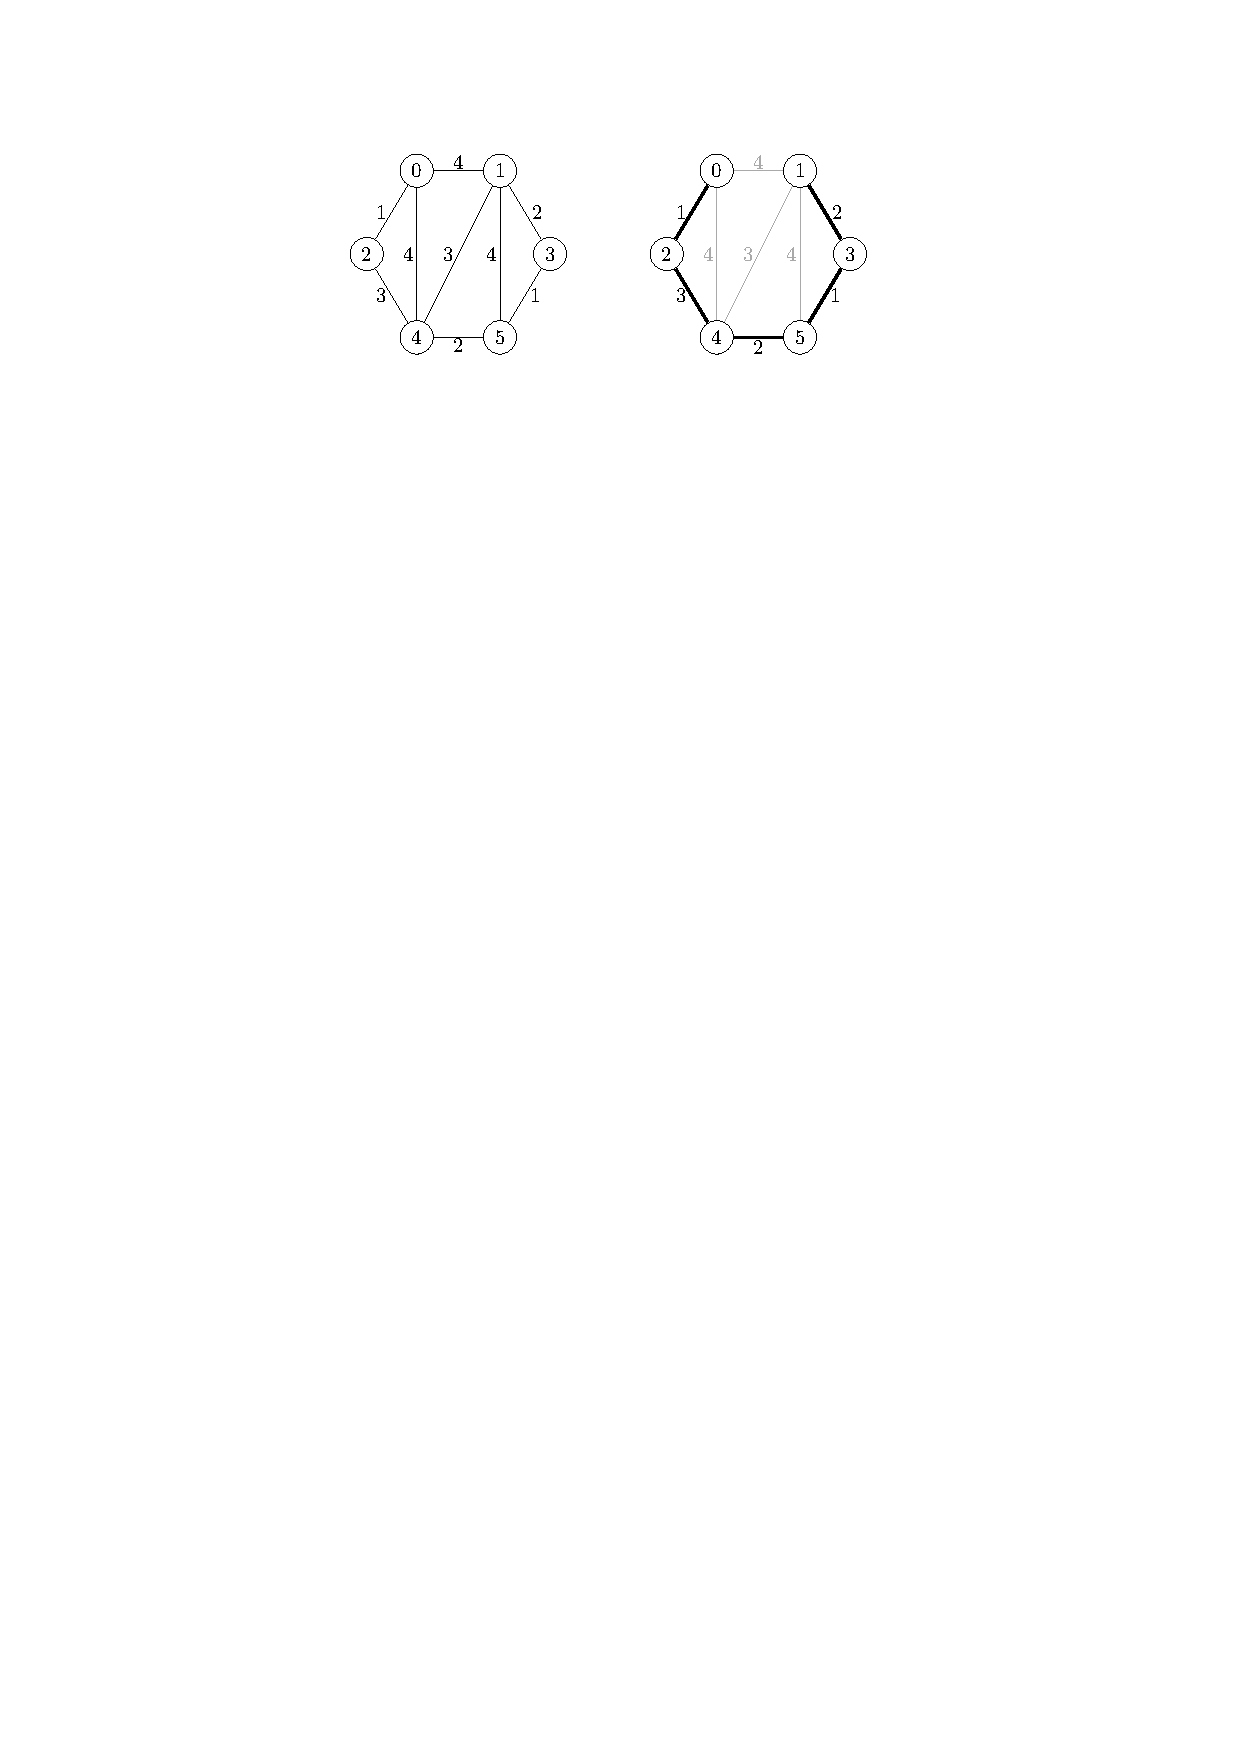
\includegraphics{graphExMST}
\end{center}
\end{Boxample}

%One should not search naively through all possible spanning trees: it is
%known that there are $n^{n-2}$ spanning trees for the complete graph
%$K_n$, for example!

We look at two simple greedy algorithms that solve the MST problem.

\section{Prim's algorithm}

%Each builds up a MST by iteratively choosing an edge greedily, that is,
%choosing one with minimum weight, subject to not obviously ruining our
%chance of extending to a spanning tree. It turns out that this simple
%approach works for the MST problem (obviously, not for all graph
%optimization problems!). There are other algorithms with better
%theoretical complexity for the MST problem, but none is as simple to
%understand.

The basic idea of  \defnfont{Prim's algorithm} is simple:
\begin{itemize}
\item Start at any vertex.
\item choose at each step an edge of minimum weight from the remaining edges ensuring that
\begin{enumerate}
\item adding the edge does not create a cycle in the subgraph built so
far; and 
\item the subgraph built so far is connected.
\end{enumerate}
\item Stop when the tree is a spanning tree.
\end{itemize}

Since the subgraph so built is acyclic and connected at each stage,  it 
is a tree.

It is also clear that the algorithm halts and as the tree grows by a node at each stage so will eventually include all nodes of $G$, that is,  be spanning. 

So the only thing that needs to be proved for correctness is that the tree has the lowest possible weight (is minimum). We will prove this but first look at the code.

Pseudocode is given in \cref{alg:primcode}. Note how similar Prim's algorithm is to Dijkstra's
The main difference is in the update formula. 
 We also store the PFS tree, which we did not
to do for Dijkstra.


\begin{algorithm}[H]
  \caption{Prim's algorithm.}
  \label{alg:primcode}
\begin{algorithmic}[1]
\Function{Prim}{weighted digraph $(G, c)$; vertex $s\in V(G)$}
	\State priority queue $Q$
	\State array $\colour[0..n-1], \pred[0..n-1]$
	\For{$u\in V(G)$}
		\State $\colour[u] \gets$ WHITE; $\pred[u] \gets NULL$ 
	\EndFor
	\State $\colour[s] \gets $ GREY
	\State $Q$.\algfont{insert}$(s, 0)$
	\While{\textbf{not} $Q$.\algfont{isEmpty}$()$}
		\State $u \gets Q$.\algfont{peek}$()$
		\For{each $x$ adjacent to $u$}
			\State $t \gets c(u, x)$
			\If{$\colour[x] = $ WHITE}
				\State $\colour[x] \gets $ GREY; $\pred[x] \gets u$
				\State $Q$.\algfont{insert}$(x, t)$
			\ElsIf{$\colour[x] = $ GREY \textbf{and} $Q$.\algfont{getKey}$(x) > t$}
				\State $Q$.\algfont{decreaseKey}$(x, t)$; $\pred[x] \gets u$
			\EndIf
		\EndFor
		\State $Q$.\algfont{delete}$()$
		\State $\colour[u] \gets $ BLACK
	\EndWhile
	\State \Return{$\pred$}
\EndFunction
\end{algorithmic}
\end{algorithm}

\begin{Boxample}
Application of Prim's algorithm on a digraph.
\begin{center}
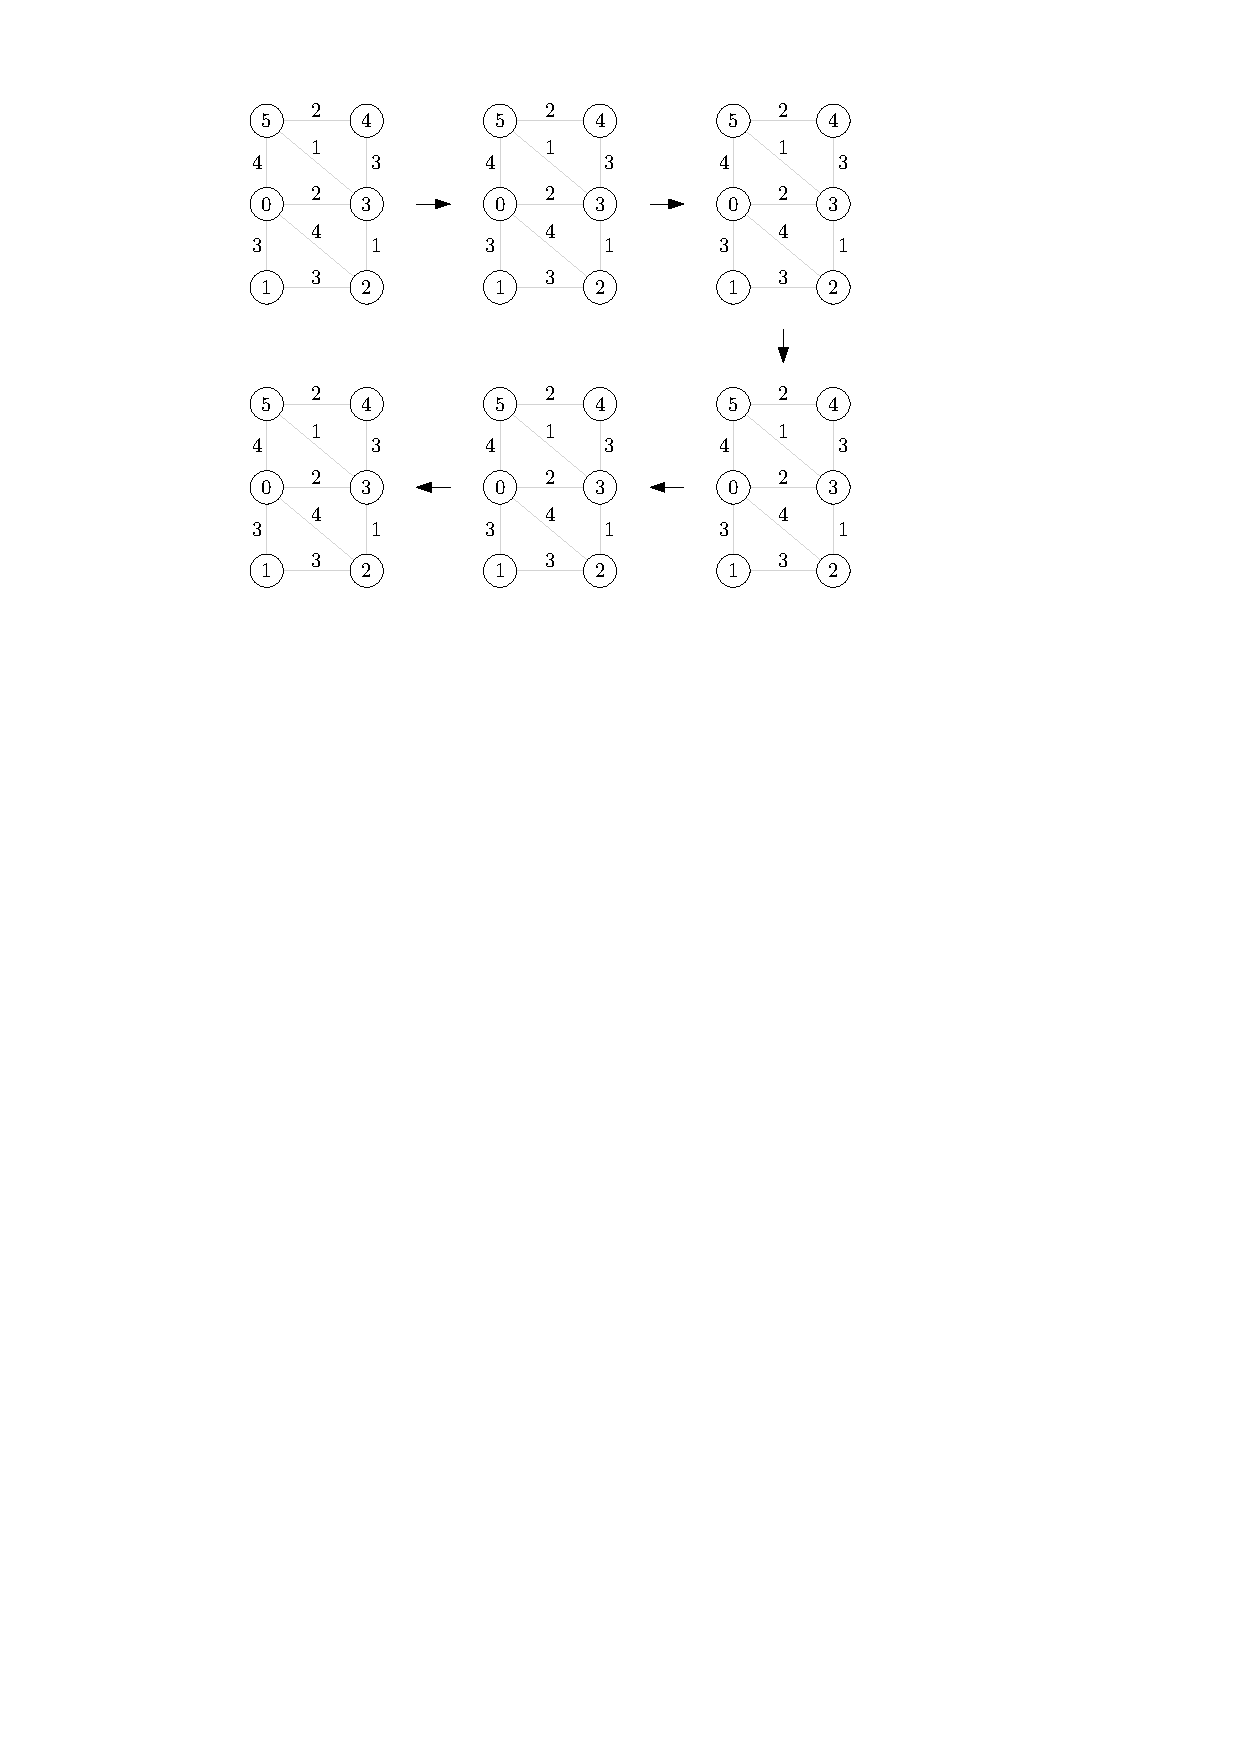
\includegraphics[width=1.0\textwidth]{PrimEx}
\end{center}
\end{Boxample}

%We now show the correctness of these algorithms. We may suppose that the
%graph is connected. If it is not, we cannot find a spanning tree anyway,
%and must be satisfied with a spanning forest. Prim's algorithm will
%terminate when it has explored the first component and must be
%restarted from a new root in another component. Kruskal's algorithm
%will find a spanning forest without modification.

\begin{Theorem}
\label{thm:prim}
Prim's algorithms is correct.
\end{Theorem}

\begin{proof}
Define a set of edges to be \emph{promising} if it can be
extended in some way to a MST. Then the empty set is promising since
some MST exists. We claim that at each step, the algorithms above have
chosen a promising set of edges. When they terminate, no further
extension of the set  is possible (by rule (a) above), and so we must
have a MST.

To prove the claim efficiently, we need a technical fact, as follows.
Suppose that $B$ is a subset of $V(G)$, not containing all the vertices
of $G$, and $T$ a promising set of edges such that no edge in $T$ leaves
$B$. In other words, either both endpoints are in $B$ or neither
endpoint is in $B$. Then if $e$ is a minimum weight edge that does leave
$B$ (it has one endpoint in $B$ and one outside) then $T\cup\{e\}$ is
also promising.

To see this fact, note that since $T$ is promising, it is contained in
some MST, $U$ say. If $e\in U$ there is nothing to prove. Otherwise,
when we add $e$ to $U$ we create exactly one cycle. There must be at
least one other edge, say $e'$, that leaves $B$, otherwise the cycle
could not close. If we remove $e'$ we obtain a new tree that spans $G$
and whose total weight is no greater than the total weight of $U$. Thus
$V$ is also a MST, and since it contains $T\cup\{e\}$, that set is
promising.

Now to prove the claim, suppose that our algorithm has maintained a
promising set $T$ of edges so far, and it has just chosen edge $e=\{u,v\}$.
If we take $B$ at each step to be the set of vertices in the tree (Prim)
or the set of vertices in the tree containing $u$ (Kruskal), then we may
apply the fact above to conclude that $T \cup \{e\}$ is promising. This
concludes the proof of correctness.
\end{proof}

\subsection{running time}

The complexity of the algorithm depends to a great extent on the data
structures used. The best known for Prim is the same as for Dijkstra,
namely $O(m + n\log n)$,

\section{Kruskal's algorithm}

\defnfont{Kruskal's algorithm} is even simpler than Prim's to state.
\begin{itemize}
\item Start with an empty set of edges.
\item choose at each step an edge of minimum weight from the remaining edges ensuring that adding the edge does not create a cycle in the subgraph built so
far. 
\item Stop when the subgraph is spanning tree.
\end{itemize}


Kruskal's algorithm maintains acyclicity, so it has a forest
at each step, and the different trees merge as the algorithm progresses.


\begin{algorithm}[H]
  \caption{Kruskal's algorithm.}
  \label{alg:kruskal}
\begin{algorithmic}[1]
\Function{Kruskal}{weighted digraph $(G, c)$}
	\State disjoint sets ADT $A$
	\State initialize $A$ with each vertex in its own set
	\State sort the edges in increasing order of cost
	\For{each edge $\{u, v\}$ in increasing cost order}
		\If{\textbf{not} $A$.\algfont{set}$(u) = A$.\algfont{set}$(v)$}
			\State add this edge
			\State $A$.\algfont{union}$(A$.\algfont{set}$(u)$, $A$.\algfont{set}$(v))$
		\EndIf
	\EndFor
	\State \Return{$A$}
\EndFunction
\end{algorithmic}
\end{algorithm}

\begin{Boxample}
Application of Kruskal's algorithm on a graph shown until an MST is found. 
Note that the edge \set{0, 2} with weight $2$ is not added, 
because $0$ and $2$ are already in the same set in $A$.
\begin{center}
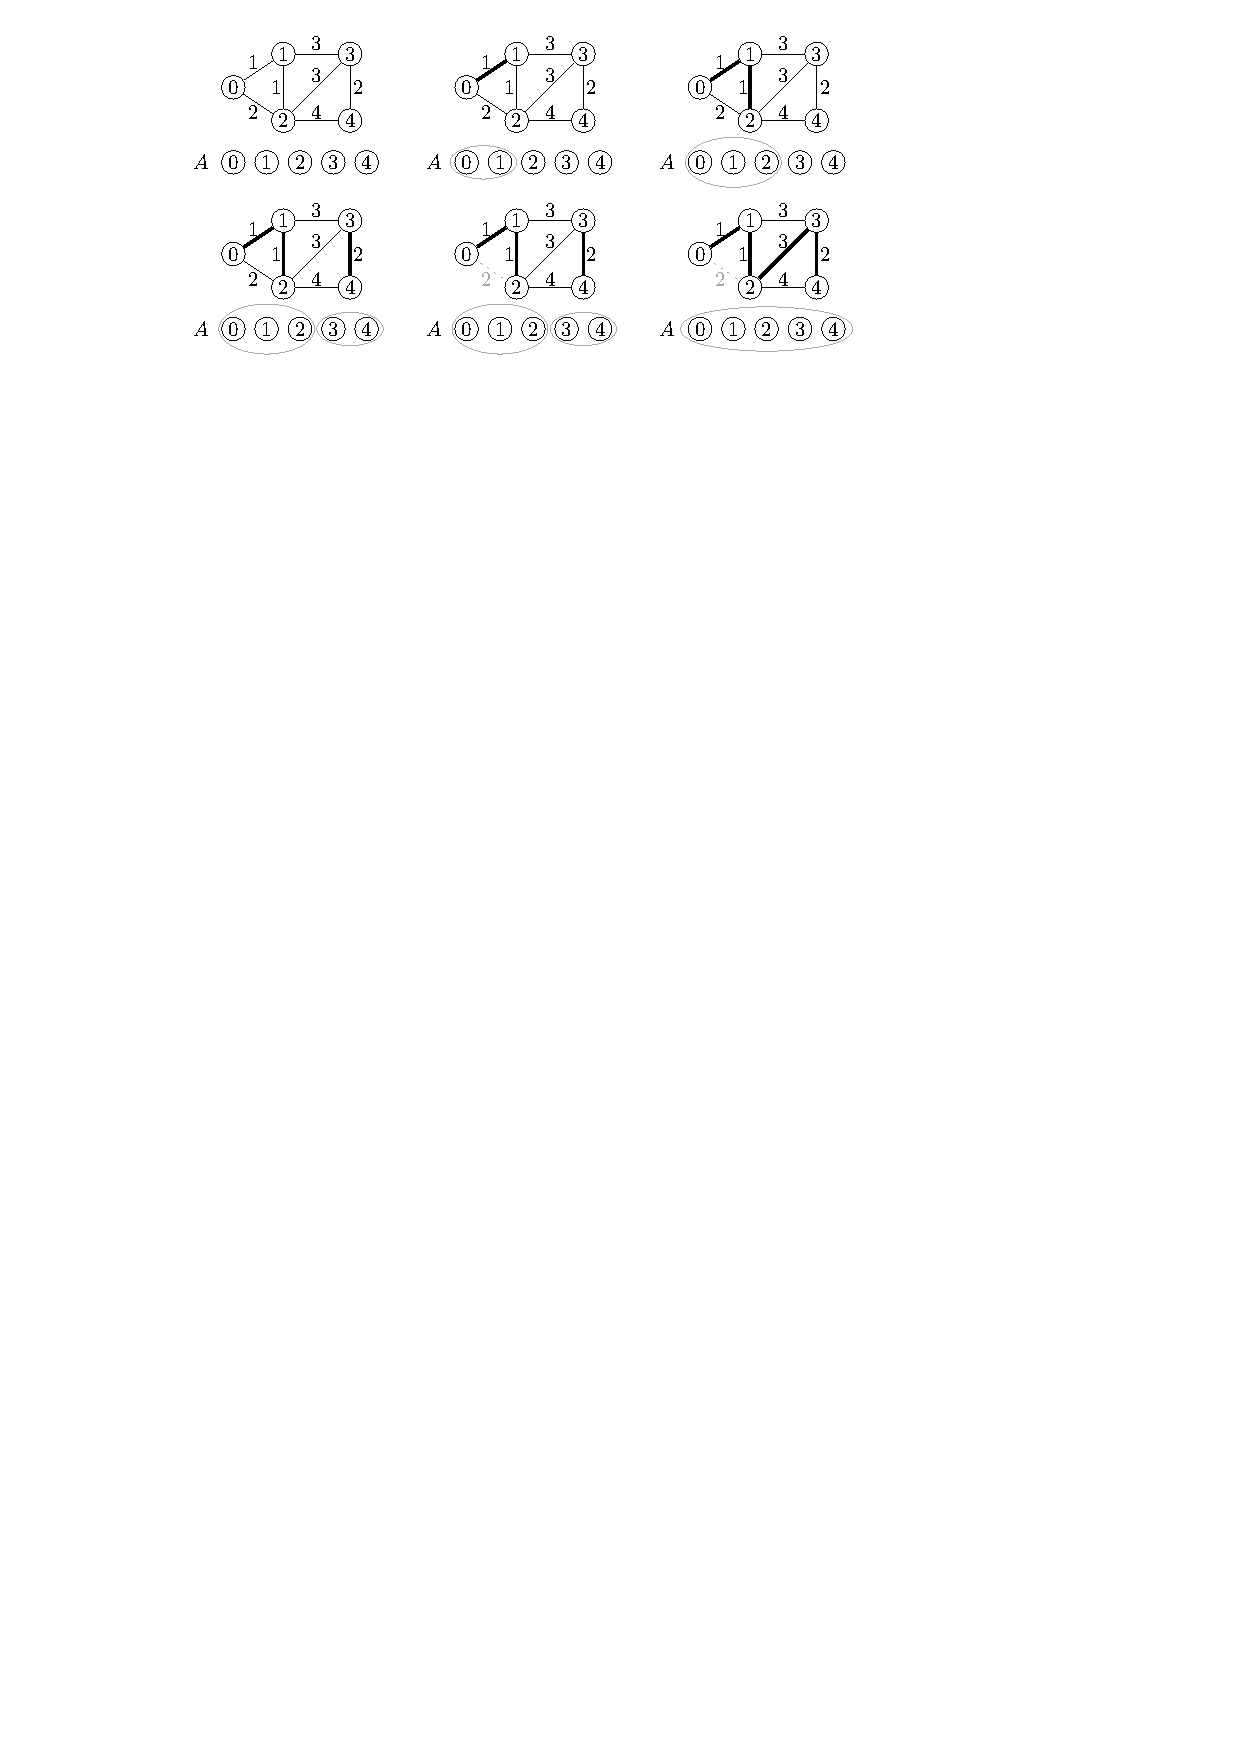
\includegraphics{KruskalEx2}
% 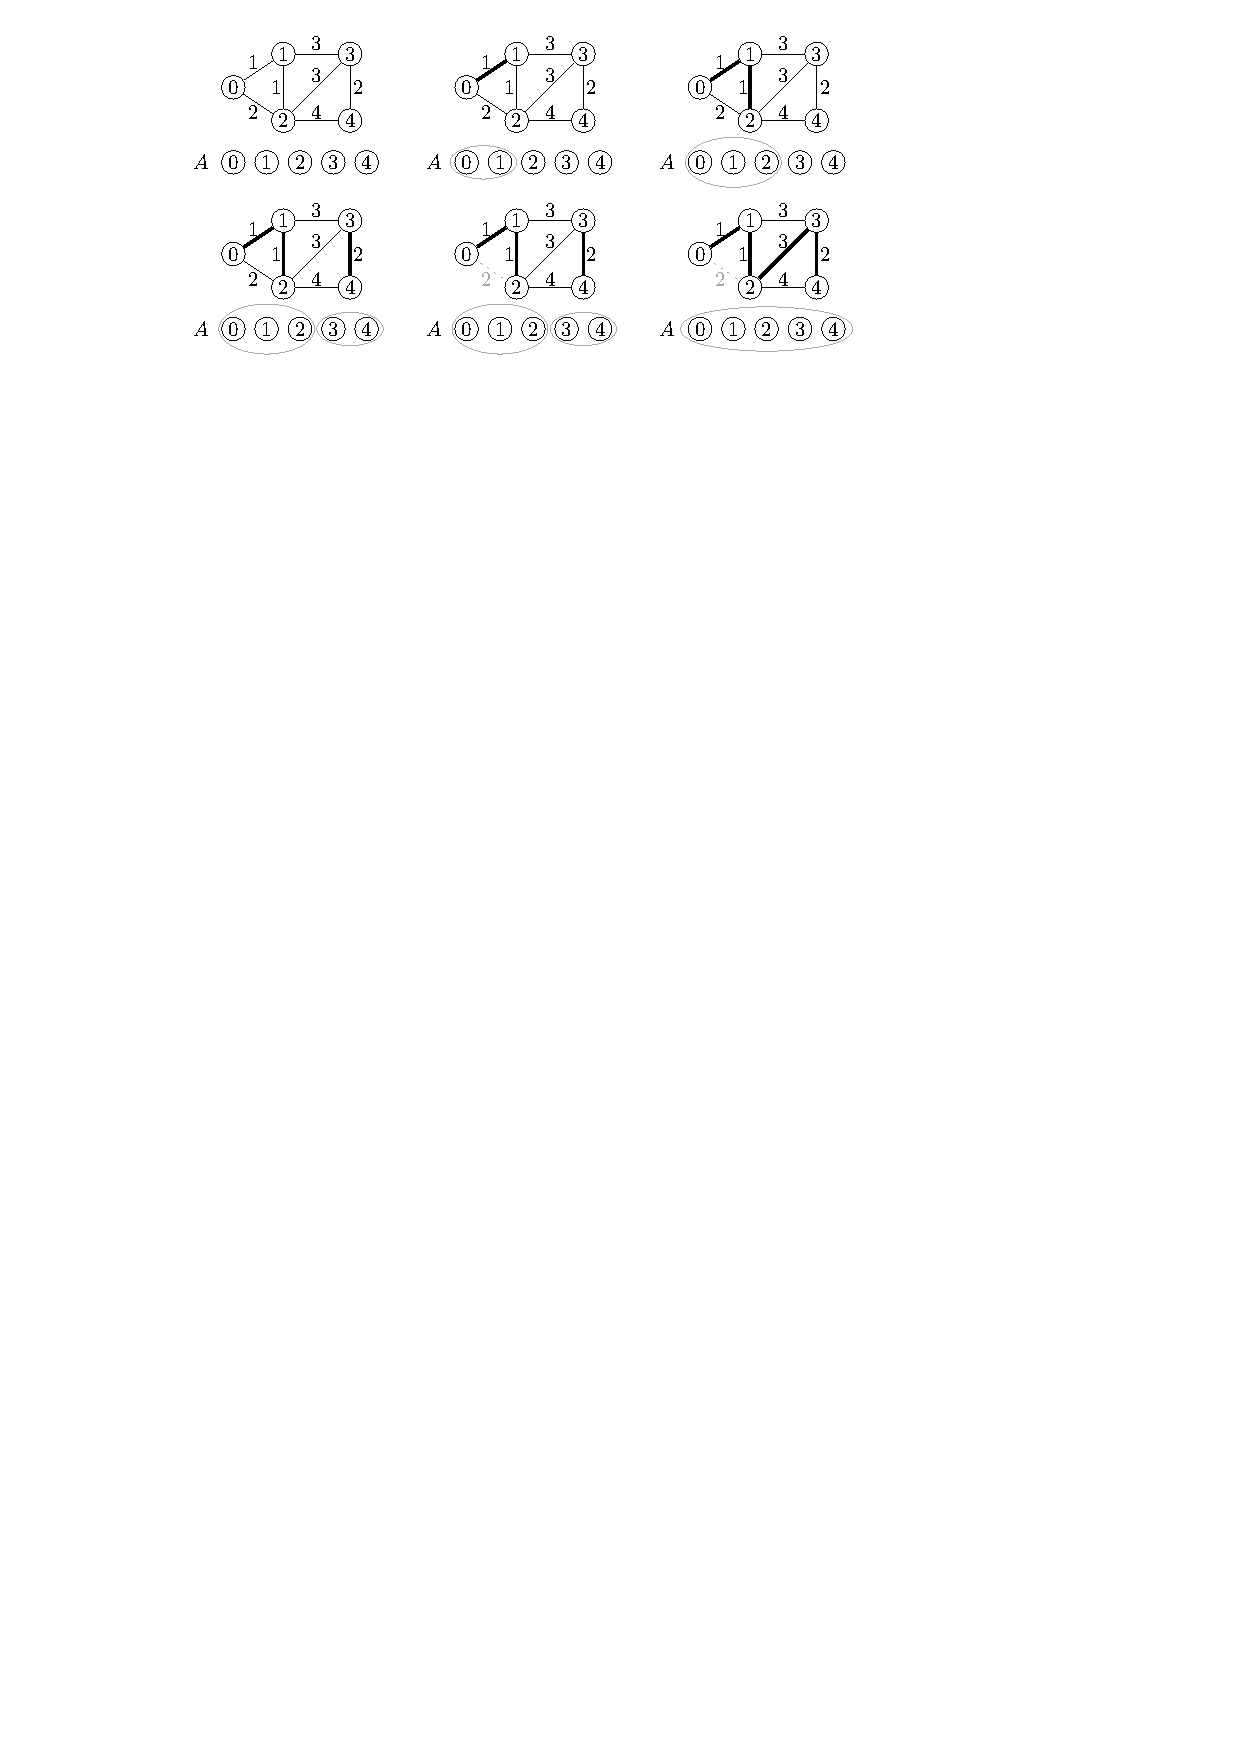
\includegraphics[width=1.0\textwidth]{KruskalEx2}
\end{center}
\end{Boxample}


In Prim's algorithm, we checked whether a cycle would be created by adding
an edge in the usual way: when exploring $\{u, v\}$ from $u$, if $v$ has
already been seen and is not the parent of $u$, then adding $\{u, v\}$
creates a cycle. With Kruskal's algorithm, we must use another method,
since the above test does not work. Both $u$ and $v$ may have been seen,
but may be in different trees.

Observe that if we try to add an edge both of whose endpoints are in
the same tree in the Kruskal forest, this will create a cycle, so the
edge must be rejected. On the other hand, if the endpoints are in two
different trees, a cycle definitely will not be created; rather, the two
trees merge into a single one, and we should accept the edge. 

We need a data structure that can handle this efficiently. All we need is to be
able to find the tree containing an endpoint, and to merge two trees. The
\defnfont{disjoint sets} or \defnfont{union-find} ADT is precisely what
is needed. It allows us to perform the \algfont{find} and \algfont{union}
operations efficiently. % (see Section~\ref{sec:app:adt-informal}).




 and for Kruskal $O(m \log n)$. The disjoint sets
ADT can be implemented in such a way that the union and find operations
in Kruskal's algorithm runs in \boldfont{almost} linear time (the exact bound
is very complicated). So if the edge weights are presorted, or can be
sorted in linear time (for example, if they are known to be integers in
a fixed range), then Kruskal's algorithm runs for practical purposes in
linear time.

\subsection*{Exercises}

\begin{Exercise} \label{ex:doMST}
Carry out each of these algorithms on the weighted
graph of \cref{fig:graphExample5}. Do the two algorithms give the
same spanning tree? 
\end{Exercise}

\begin{Exercise} \label{ex:spanning-tree}
Prove the assertion made above that when Kruskal's or Prim's algorithm 
terminates, the current set of edges forms a spanning tree.
\end{Exercise}

\begin{Exercise}\label{ex:silly-MST}
Consider the following algorithm for the MST problem. Repeatedly delete
edges from a connected graph $G$, at each step choosing the most
expensive edge we can, subject to maintaining connectedness. Does it
solve the MST problem sometimes? always?
\end{Exercise}

\chapter{Hard graph problems}%------------------------------------------------
\label{sec:hardgraph}
We have presented several efficient algorithms for some common digraph
problems. All of these algorithms have running time bounded above by a low
degree polynomial in the size of the input. However, there are many
essential problems that currently do not have known polynomial-time
algorithms (so-called \defnfont{NP-hard} problems). Some examples
are:
\begin{itemize}
\item finding the longest path between two nodes of
a digraph;
\item finding a $k$-colouring of a graph, for fixed $k\geq
3$;
\item finding a cycle that passes through all the vertices of
a graph (a \defnfont{Hamiltonian cycle});
\item finding a
minimum weight path that passes through all the vertices of a weighted
digraph (the \defnfont{travelling salesperson problem} or TSP);
\item finding the largest \defnfont{independent set} in a graph --- that is, 
a subset of vertices no two of which are connected by an edge;
\item finding the smallest 
\defnfont{vertex cover} of a graph---that is, a special subset of
vertices so that each vertex of the graph is adjacent to one in that
subset. (However, from Exercise~\ref{ex:konig}, this problem 
is polynomial-time solvable when restricted to bipartite graphs.)

\end{itemize}

Investigating these problems is an active research area in computer
science. In many cases the only approach known is essentially to try
all possibilities, with some rules that prevent the listing of obviously
hopeless ones. In some special cases (for example, graphs that are 
\defnfont{planar} (they can be drawn in the plane without edges crossing) 
or are in some sense ``close to" trees, much faster algorithms can be developed.

\subsection*{Exercises}

\begin{Exercise}\label{exr:tsp}
Find a Hamiltonian cycle of the graph in Exercise~\ref{ex:dijk-SI}. Try to solve
the TSP for this graph.
\end{Exercise}

\begin{Exercise}\label{exr:indset}
What is the exact relation between the independent set and vertex cover problems?
\end{Exercise}

%\section{Notes}
%
%Dijkstra's algorithm was proposed by E. W. Dijkstra in 1959.
%The Bellman--Ford algorithm was proposed independently by R.
%Bellman (1958) and L. R. Ford, Jr (1956). Floyd's algorithm was developed in 
%1962 by R. W. Floyd. Prim's algorithm was presented by R. C. Prim in 1957
%and reinvented by E. W. Dijkstra in 1959, but had been previously introduced by 
%V. Jarnik in 1930. Kruskal's algorithm was introduced by J. Kruskal in 1956.

